% Version control information:
%$HeadURL: https://practicas-PASW.googlecode.com/svn/trunk/anova_1_factor/anova_1_factor.tex $
%$LastChangedDate: 2010-09-27 16:37:11 +0200 (lun, 27 sep 2010) $
%$LastChangedRevision: 3 $
%$LastChangedBy: asalber $
%$Id: anova_1_factor.tex 3 2010-09-27 14:37:11Z asalber $

\chapter{ANOVA de Dos o Más Factores, ANOVA de Medidas Repetidas y ANCOVA}

\medskip
\section{Fundamentos teóricos}

Como ya se vio en una práctica anterior, el \emph{Análisis de la Varianza de un Factor},
\emph{ANOVA} o también \emph{ANOVA de una Vía}, es una técnica
estadística de contraste de hipótesis cuyo propósito es estudiar
el efecto de la aplicación de varios \emph{niveles} (también
llamados \emph{tratamientos}) de una variable aleatoria
cualitativa, llamada \emph{factor} o \emph{vía}, en una variable cuantitativa,
llamada \emph{respuesta}. Si se supone que la variable cualitativa independiente,
es decir el factor, presenta $k$ niveles diferentes, entonces para comparar
las $k$ medias de la variable respuesta según los
diferentes niveles del factor se realiza un contraste de
hipótesis, cuya hipótesis nula, $H_0$, es que la variable
respuesta tiene igual media en todos los niveles, mientras que la
hipótesis alternativa, $H_1$, es que hay diferencias
estadísticamente significativas en al menos dos de las medias. Dicho contraste de hipótesis se basa en la comparación de dos
estimadores de la varianza total de los datos de la variable
respuesta; de ahí procede el nombre de esta técnica: \emph{ANOVA}
(Analysis of Variance).

No obstante, en muchos problemas aparece no ya un único factor que permite clasificar los individuos de la muestra en $k$ diferentes
niveles, sino que pueden presentarse dos o más factores que permiten clasificar a los individuos de la muestra en múltiples grupos según
diferentes criterios, que se pueden analizar para ver si hay o no diferencias significativas entre las medias de la variable respuesta. Para
tratar con este tipo de problemas surge el \emph{ANOVA de Dos o Más Factores} (o también \emph{ANOVA de Dos o Más Vías}) como una
generalización del proceso de un factor, que además de permitir el análisis de la influencia de cada uno de los factores por separado
también hace posible el estudio de la \emph{interacción} entre ellos.

Por otra parte, también son frecuentes los problemas en los que se toma más de una medida de una variable cuantitativa (respuesta) en cada
sujeto de la muestra, y se procede al análisis de las diferencias entre las diferentes medidas. Si sólo se toman dos, el procedimiento
adecuado es la T de Student de datos pareados, o su correspondiente no paramétrico, el test de Wilcoxon; pero si se han tomado tres o más
medidas, el test paramétrico correspondiente a la T de Student de datos pareados es el \emph{ANOVA de Medidas Repetidas}.

Incluso también se puede dar el caso de un problema en el que se analice una misma variable cuantitativa medida en varias ocasiones en cada
sujeto de la muestra pero teniendo en cuenta a la vez la influencia de uno, dos o más factores que permiten clasificar a los individuos en
varios subgrupos diferentes. En definitiva, pueden aparecer problemas donde a la par que un ANOVA de medidas repetidas se requiera realizar
un ANOVA de dos o más vías.

Por último, la situación más compleja que se puede plantear en el análisis de una respuesta cuantitativa se presenta cuando, añadida a
medidas repetidas y dos o más vías o factores de clasificación, se tienen una o más variables cuantitativas, llamadas \emph{Covariables},
que se piensa que pueden influir en la variable respuesta. Se procede entonces a realizar un \emph{ANCOVA} o \emph{Análisis de Covarianza},
con el que se pretende analizar la influencia de los factores y también ver si hay diferencias entre las medidas repetidas pero habiendo
eliminado previamente la influencia (variabilidad) debida a la presencia de las covariables que se pretenden controlar.


\subsection{ANOVA de dos o más factores}

\subsubsection{ANOVA de dos factores con dos niveles cada factor}

Para entender qué es un ANOVA de dos o más factores, conviene partir de un caso sencillo con dos factores y dos niveles en cada factor. Por
ejemplo, se puede plantear un experimento con individuos que siguen o no una dieta (primer factor: dieta, con dos niveles: sí y no), y que a
su vez toman o no un determinado fármaco (segundo factor: fármaco, con dos niveles: sí y no) para reducir su peso corporal (variable
respuesta numérica: reducción del peso corporal expresada en Kg). En esta situación, se generan cuatro grupos diferentes: los que no hacen
dieta ni toman fármaco (No-No), los que no hacen dieta pero sí toman fármaco (No-Sí), los que hacen dieta y no toman fármaco (Sí-No), y los
que hacen dieta y toman fármaco (Sí-Sí). Y se pueden plantear tres efectos diferentes:

\begin{itemize}

\item El de la dieta: viendo si hay o no diferencias significativas en los Kg perdidos entre los individuos que la han seguido y los que no.

\item El del fármaco: viendo si hay o no diferencias significativas en los Kg perdidos entre los individuos que lo han tomado y los que no.

\item El de la interacción: viendo si el efecto combinado de dieta y fármaco es diferente del que tendrían sumando sus efectos por separado, y entonces se diría que sí que hay interacción; o si por el contrario el efecto de la combinación de dieta y fármaco es el mismo que la suma de los efectos por separado, y entonces se diría que no hay interacción. A su vez, si hay interacción se puede dar en dos sentidos: si la combinación de dieta y fármaco ha hecho perder más kilos a los pacientes de los que cabría esperar con la suma de dieta y fármaco por separado, entonces la interacción de ambos factores ha actuado en sinergia con los mismos, mientras que si la combinación ha hecho perder menos kilos de los que cabría esperar con dieta y fármaco por separado, entonces la interacción ha actuado en antagonismo con ambos.

\end{itemize}

Siguiendo con el ejemplo, supongamos que la tabla que aparece a continuación refleja la media de Kg perdidos dentro de cada uno de los grupos comentados. Por simplificar el ejemplo, no se reflejan los Kg en cada individuo con la consiguiente variabilidad de los mismos, pero el ANOVA de dos vías sí que tendría en cuenta esa variabilidad para poder hacer inferencia estadística, plantear contrastes de hipótesis y calcular sus correspondientes p-valores.

\begin{center}
\begin{tabular}{|l|l|l|}
\cline{2-3}
\multicolumn{1}{c|}{} & \multicolumn{1}{c|}{Fármaco No} & \multicolumn{1}{c|}{Fármaco Sí} \\
\hline
\multicolumn{1}{|c|}{Dieta No} & \multicolumn{1}{c|}{0} & \multicolumn{1}{c|}{5} \\
\hline
\multicolumn{1}{|c|}{Dieta Sí} & \multicolumn{1}{c|}{3} & \multicolumn{1}{c|}{8} \\
\hline
\end{tabular}
\end{center}

Si los resultados obtenidos fuesen los de la tabla anterior, se diría que no hay interacción entre fármaco y dieta, ya que el efecto del
fármaco en el grupo de los que no hacen dieta ha hecho perder 5 Kg en media a los individuos, el efecto de la dieta en el grupo de los que
no toman fármaco les ha hecho perder 3 Kg en media, y el efecto combinado de dieta y fármaco ha hecho perder 8 Kg con respecto a los que no
hacen dieta y tampoco toman fármaco. Estos 8 Kg son iguales a la suma de 3 y 5, es decir iguales a la suma de los efectos de los factores
por separado, sin ningún tipo de interacción (de término añadido) que cambie el resultado de la suma.

Con las medias de los cuatro grupos que se generan en el cruce de los dos factores, cada uno con dos niveles (2x2), se representan los
gráficos de medias que aparecen más adelante. En estos gráficos, cuando no hay interacción las rectas que unen las medias correspondientes a
un mismo nivel de uno de los factores son paralelas dentro de cierto margen de variabilidad.

\begin{figure}[h!]
\begin{center}
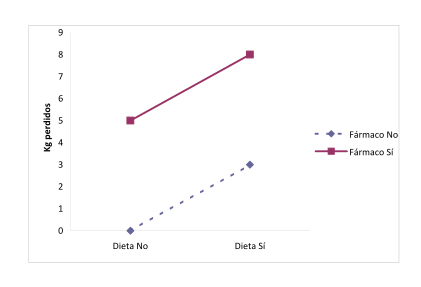
\includegraphics[scale=0.6]{anova_2_factores/img/sininteraccion}
\caption{Gráfico de medias de dos factores sin interacción}
\end{center}
\end{figure}

Por el contrario, también podría obtenerse una tabla en la que la suma de los efectos por separado fuese menor que el efecto combinado de dieta y fármaco:

\begin{center}
\begin{tabular}{|l|l|l|}
\cline{2-3}
\multicolumn{1}{c|}{} & \multicolumn{1}{c|}{Fármaco No} & \multicolumn{1}{c|}{Fármaco Sí} \\
\hline
\multicolumn{1}{|c|}{Dieta No} & \multicolumn{1}{c|}{0} & \multicolumn{1}{c|}{5} \\
\hline
\multicolumn{1}{|c|}{Dieta Sí} & \multicolumn{1}{c|}{3} & \multicolumn{1}{c|}{12} \\
\hline
\end{tabular}
\end{center}

En este caso, dejando al margen las variabilidad dentro de cada uno de los grupos y suponiendo que la misma es lo suficientemente pequeña
como para que las diferencias sean significativas, los 8 Kg en media que se perderían al sumar los efectos por separado de dieta y fármaco
son menores que los 12 que, en media, han perdido los individuos que han tomado el fármaco y han seguido la dieta a la vez. Por lo tanto, se
ha producido una interacción de los dos factores que, al unirlos, ha servido para potenciar sus efectos por separado. Dicho de otra forma,
para explicar el resultado final de los individuos que han tomado el fármaco y también han seguido la dieta habría que introducir un nuevo
término en la suma, el término de interacción, que contribuiría con 4 Kg de pérdida añadidos a los 8 Kg que se perderían considerando
simplemente la suma de dieta y fármaco. Como este nuevo término contribuye a aumentar la pérdida que se obtendría al sumar los efectos por
separado de ambos factores, se trataría de un caso de interacción en sinergia con los dos factores de partida.

\begin{figure}[h!]
\begin{center}
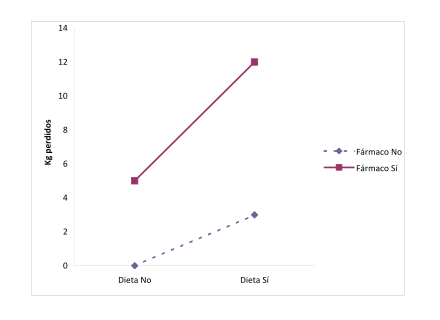
\includegraphics[scale=0.6]{anova_2_factores/img/coninteraccion1}
\caption{Gráfico de medias de dos factores con interacción sinérgica.}
\end{center}
\end{figure}

Por último, también se podría obtener una tabla en la que la suma de los efectos por separado fuese mayor que el efecto combinado de los dos
factores:

\begin{center}
\begin{tabular}{|l|l|l|}
\cline{2-3}
\multicolumn{1}{c|}{} & \multicolumn{1}{c|}{Fármaco No} & \multicolumn{1}{c|}{Fármaco Sí} \\
\hline
\multicolumn{1}{|c|}{Dieta No} & \multicolumn{1}{c|}{0} & \multicolumn{1}{c|}{5} \\
\hline
\multicolumn{1}{|c|}{Dieta Sí} & \multicolumn{1}{c|}{3} & \multicolumn{1}{c|}{4} \\
\hline
\end{tabular}
\end{center}

Igualmente, en este nuevo ejemplo los 8 Kg en media que se perderían al sumar los efectos por separado de los dos factores son mayores que
los 4 que en realidad pierden, en media, los individuos que han seguido la dieta y utilizado el fármaco. Por lo tanto, para explicar el
resultado obtenido en el grupo de los que toman el fármaco y siguen la dieta habría que introducir un término añadido a la suma de efectos
sin más, que se restaría a los 8 Kg hasta dejarlos en 4 Kg. Se trataría de un caso de interacción en antagonismo con los dos factores de
partida.

\begin{figure}[h!]
\begin{center}
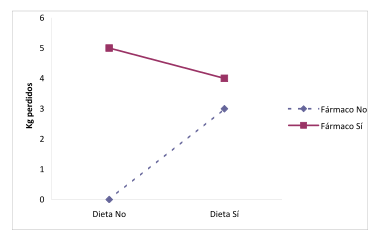
\includegraphics[scale=0.6]{anova_2_factores/img/coninteraccion2}
\caption{Gráfico de medias de dos factores con interacción antagónica.}
\end{center}
\end{figure}

En realidad, la interacción también puede producirse en sinergia con uno de los factores y en antagonismo con el otro, ya que a veces los
dos factores pueden producir un efecto con signo contrario. Por ejemplo, al hablar del factor dieta, se tiende a pensar que se trata de una
dieta que sirve para bajar el peso, pero también cabe plantearse un experimento con personas que siguen una dieta de alto contenido calórico
que en principio debería hacerles subir peso y ver qué evolución siguen cuando a la vez toman un fármaco para bajarlo.

Como puede deducirse fácilmente de las tablas y gráficas anteriores, la presencia de interacción implica que la diferencia entre las medias
de los dos grupos dentro de un mismo nivel de uno de los factores no es la misma que para el otro nivel. Por ejemplo, en la segunda tabla,
la diferencia entre las medias de Kg perdidos entre los que sí que toman el fármaco y los que no lo toman vale: 5-0=5 Kg en los que no hacen
dieta, y 12-3=9 Kg en los que sí que hacen dieta. Lo cual gráficamente se traduce en que la pendiente de la recta que une las medias dentro
del grupo de los que sí que toman el fármaco es diferente de la pendiente que une las medias dentro del grupo de los que no lo toman. En las
ideas anteriores se basará el planteamiento del contraste de hipótesis para ver si la interacción ha resultado o no significativa.

Como ya se ha comentado, en cualquiera de las tablas anteriores se podrían analizar tres efectos diferentes: el de la dieta, el del fármaco
y el de la interacción de dieta con fármaco; lo cual, en términos matemáticos, se traduce en tres contrastes de hipótesis diferentes:

\begin{enumerate}

\item Efecto de la dieta sobre la cantidad de peso perdido:

$H_0: \mu_{\text{con dieta}}=\mu_{\text{sin dieta}}$

$H_1: \mu_{\text{con dieta}}\neq\mu_{\text{sin dieta}}$

\item Efecto del fármaco sobre la cantidad de peso perdido:

$H_0: \mu_{\text{con fármaco}}=\mu_{\text{sin fármaco}}$

$H_1: \mu_{\text{con fármaco}}\neq\mu_{\text{sin fármaco}}$

\item Efecto de la interacción entre dieta y fármaco, que a su vez se puede plantear de dos formas equivalentes:

\begin{enumerate}
\item Viendo si dentro dentro de los grupos definidos en función de la dieta la diferencia de Kg perdidos entre los que toman fármaco y los que no lo toman es la misma:

$H_0: (\mu_{\text{con fármaco}}-\mu_{\text{sin fármaco}})_{\text{sin dieta}}=(\mu_{\text{con fármaco}}-\mu_{\text{sin fármaco}})_{\text{con dieta}}$

$H_1: (\mu_{\text{con fármaco}}-\mu_{\text{sin fármaco}})_{\text{sin dieta}}\neq(\mu_{\text{con fármaco}}-\mu_{\text{sin fármaco}})_{\text{con dieta}}$

\item Viendo si dentro de los grupos definidos en función del fármaco la diferencia de Kg perdidos entre los que hacen dieta y los que no la hacen es la misma:

$H_0: (\mu_{\text{con dieta}}-\mu_{\text{sin dieta}})_{\text{sin fármaco}}=(\mu_{\text{con dieta}}-\mu_{\text{sin dieta}})_{\text{con fármaco}}$

$H_1: (\mu_{\text{con dieta}}-\mu_{\text{sin dieta}})_{\text{sin fármaco}}\neq(\mu_{\text{con dieta}}-\mu_{\text{sin dieta}})_{\text{con fármaco}}$
\end{enumerate}
\end{enumerate}

Aunque los detalles matemáticos más precisos sobre cómo el ANOVA de dos o más vías da respuesta a los contrastes expuestos quedan fuera del
nivel de esta práctica, la idea general es sencilla y muy parecida a la explicada con más detalle en la práctica de ANOVA de una vía.  En el
ANOVA de una vía, la variabilidad total de los datos, expresada como suma de distancias al cuadrado con respecto a la media global (llamada
Suma de Cuadrados Total), se descompone en dos diferentes fuentes de variabilidad: las distancias al cuadrado de los datos de cada grupo con
respecto a la media del grupo, \emph{Suma de Cuadrados Intra}, más las distancias al cuadrado entre las diferentes medias de los grupos y la
media general, \emph{Suma de Cuadrados Inter}. La suma de cuadrados intra-grupos es también llamada \emph{Variabilidad Residual} o
\emph{Suma de Cuadrados Residual}, ya que su cuantía es una medida de la dispersión residual, remanente incluso después de haber dividido
los datos en grupos. Estas sumas de cuadrados, una vez divididas por sus correspondientes grados de libertad, generan varianzas llamadas
\emph{Cuadrados Medios}, y el cociente de cuadrados medios (cuadrado medio inter dividido entre cuadrado medio intra) bajo la hipótesis nula
de igualdad de medias en todos los grupos sigue una distribución \emph{F} de Fisher que se puede utilizar para calcular un $p$-valor del
contraste de igualdad de medias. En el ANOVA de dos factores, en lugar de dos fuentes de variabilidad tenemos cuatro: una por el primer
factor, otra por el segundo, otra por la interacción y otra más que contempla la variabilidad residual o variabilidad intragrupos. En el
ejemplo anterior, las cuatro fuentes de variabilidad son:


\begin{enumerate}
\item La debida al primer factor: la dieta.
\item La debida al segundo factor: el fármaco.
\item La debida a la interacción entre ambos.
\item La residual.
\end{enumerate}

Las tres primeras fuentes de variabilidad llevan asociadas sus correspondientes sumas de cuadrados, similares a la suma de cuadrados inter
del ANOVA de una vía, mientras que la variabilidad residual lleva asociada su suma de cuadrados residual, similar a la suma de cuadrados
intra del ANOVA de una vía. Dividiendo las sumas de cuadrados entre sus respectivos grados de libertad se obtienen varianzas, que divididas
entre la varianza residual generan, bajo la hipótesis nula de igualdad de medias, valores \emph{f} de la distribución \emph{F} de Fisher que
pueden utilizarse para calcular el p-valor del correspondiente contraste.

Lo anterior se resume en forma de tabla de un ANOVA de dos vías, considerando un primer factor con $k_1$ niveles, un segundo factor con
$k_2$ niveles y un total de datos $n$. Si se denomina F1 al primer factor, F2 al segundo, I a la interacción y R al residual, la tabla de un
ANOVA de dos vías tiene la siguiente forma:

\begin{center}
\renewcommand{\arraystretch}{2}
\begin{tabular}{|l|l|l|l|l|l|}
\hline
\multicolumn{1}{|c|}{Fuente} & \multicolumn{1}{c|}{Suma Cuad} & \multicolumn{1}{c|}{Grad Lib} & \multicolumn{1}{c|}{Cuad Medios} & \multicolumn{1}{c|}{f} & \multicolumn{1}{c|}{$p$-valor} \\
\hline
\multicolumn{1}{|c|}{F1} & \multicolumn{1}{c|}{$SF1$} & \multicolumn{1}{c|}{$GF1=k_1-1$} & \multicolumn{1}{c|}{$CF1=\dfrac{{SF1}}{{GF1}}$} & \multicolumn{1}{c|}{$f1=\dfrac{{CF1}}{{CR}}$} & \multicolumn{1}{c|}{$P(F>f1)$} \\
\hline
\multicolumn{1}{|c|}{F2} & \multicolumn{1}{c|}{$SF2$} & \multicolumn{1}{c|}{$GF2=k_2-1$} & \multicolumn{1}{c|}{$CF2=\dfrac{{SF2}}{{GF2}}$} & \multicolumn{1}{c|}{$f2=\dfrac{{CF2}}{{CR}}$} & \multicolumn{1}{c|}{$P(F>f2)$} \\
\hline
\multicolumn{1}{|c|}{I} & \multicolumn{1}{c|}{$SI$} & \multicolumn{1}{c|}{$GI=GF1 \cdot GF2$} & \multicolumn{1}{c|}{$CI=\dfrac{{SI}}{{GI}}$} & \multicolumn{1}{c|}{$fI=\dfrac{{CI}}{{CR}}$} & \multicolumn{1}{c|}{$P(F>fI)$} \\
\hline
\multicolumn{1}{|c|}{R} & \multicolumn{1}{c|}{$SR$} & \multicolumn{1}{c|}{$GR=n-1-GF1-GF2-GI$} & \multicolumn{1}{c|}{$CR=\dfrac{{SR}}{{GR}}$} & \multicolumn{1}{c|}{} & \multicolumn{1}{c|}{} \\
\hline
\multicolumn{1}{|c|}{Total} & \multicolumn{1}{c|}{$ST$} & \multicolumn{1}{c|}{$GT=n-1$} & \multicolumn{1}{c|}{} & \multicolumn{1}{c|}{} & \multicolumn{1}{c|}{} \\
\hline
\end{tabular}
\end{center}

Una vez obtenida la tabla, habitualmente mediante un programa de estadística para evitar realizar la gran cantidad de cálculos que conlleva
(los distintos programas pueden proporcionar tablas ligeramente diferentes a la expuesta en esta práctica, en las que pueden aparecer filas
añadidas cuya interpretación dependerá del programa utilizado), el siguiente paso es la interpretación de los $p$-valores obtenidos en cada
uno de los factores y en la interacción. Para ello, resulta clave el $p$-valor de la interacción porque condicionará completamente el
análisis:
\begin{itemize}
\item Si la interacción no ha resultado significativa ($p$-valor de la interacción mayor que el nivel de significación, habitualmente
$0.05$), se puede considerar por separado la actuación de los dos factores y ver si hay o no diferencias significativas en sus niveles
atendiendo al $p$-valor que aparece en la tabla para cada uno de ellos. Por ejemplo, en la primera de las tablas del análisis de Kg perdidos
en función de la dieta y el fármaco, se obtendría que la interacción no es significativa, lo cual implicaría que habría que analizar el
efecto de los factores por separado. Para ello, se acudiría al $p$-valor del factor dieta y si es menor que el nivel de significación
fijado, entonces el factor dieta habría resultado significativo, lo cual quiere decir que habría diferencias significativas (más allá de las
asumibles por azar) entre los Kg perdidos por los individuos que hacen dieta y los que no; y todo ello, independientemente de si los
individuos están tomando o no el fármaco, ya que no hay una interacción significativa que ligue los resultados de la dieta con el fármaco.
Igualmente, con el factor fármaco, se acudiría a su $p$-valor y se vería si hay o no diferencias significativas entre los Kg perdidos por
los que toman el fármaco y los que no lo hacen, independientemente de si siguen o no la dieta.
\item Si la interacción ha resultado significativa ($p$-valor de la interacción menor que el nivel de significación, habitualmente $0.05$),
no se puede considerar por separado la actuación de los dos factores, la presencia de uno de los factores condiciona lo que sucede en el
otro y el análisis de diferencias debidas al segundo factor debe realizarse por separado dentro de cada uno de los niveles del primero; y a
la inversa, el análisis de diferencias debidas al primero debe realizarse por separado dentro de cada uno de los niveles del segundo. Por
ejemplo, en la segunda de las tablas del análisis de Kg perdidos en función de la dieta y el fármaco, muy probablemente se obtendría que la
interacción sí que es significativa, con lo cual no habría un único efecto del fármaco: en el grupo de los que no toman el fármaco, la
diferencia de Kg perdidos entre los que sí que hacen dieta y los que no  la hacen no sería la misma que en el grupo de los que sí que toman
el fármaco. E igualmente, tampoco habría un único efecto de la dieta: en el grupo de los que no hacen dieta, la diferencia de Kg perdidos
entre los que sí que toman el fármaco y los que no lo hacen no sería la misma que en el grupo de los que sí que hacen dieta.
\end{itemize}

Una aclaración final importante es que en ningún caso un ANOVA de dos factores con dos niveles en cada vía equivale a hacer por separado una
T de Student de datos independientes en cada uno de los factores. Ni siquiera en el caso de que no haya interacción el $p$-valor que se
obtiene en cada uno de los dos factores coincide con el que se obtendría en la comparación de los niveles mediante la T de Student. El ANOVA
de dos factores es una técnica multivariante que cuantifica la influencia de cada una de las variables independientes en la variable
dependiente después de haber eliminado la parte de la variabilidad que se debe a las otras variables independientes que forman parte del
modelo. En el ejemplo de los Kg perdidos, no sería lo mismo analizar la influencia de la variable dieta después de eliminar la variabilidad
explicada mediante la variable fármaco e incluso la interacción entre dieta y fármaco, que es lo que haría el ANOVA de dos factores, que
analizar simplemente la influencia de la variable dieta sin más, o fármaco sin más, que es lo que podríamos hacer mediante una T de Student
de datos independientes. Tampoco el análisis de la interacción en el ANOVA de dos factores equivale a realizar un ANOVA de una vía
considerando una nueva variable independiente con cuatro categorías diferentes (1:Sí-Sí, 2:Sí-No, 3:No-Sí, 4:No-No), por el mismo motivo:
las conclusiones del ANOVA de dos vías hay que entenderlas en el contexto de una técnica multivariante en que la importancia de cada
variable independiente se obtiene después de eliminar de los datos la variabilidad debida a las demás.


\subsubsection{ANOVA de dos factores con tres o más niveles en algún factor}
El planteamiento y resolución de un ANOVA de dos factores con tres o más niveles en algún factor es muy parecido al ya expuesto de dos
niveles en cada factor. Únicamente cambian ligeramente las hipótesis nulas planteadas en los factores en las que habría que incluir la
igualdad de tantas medias como niveles tenga el factor analizado, y las alternativas en las que se supone que alguna de las medias es
diferente. En cuanto a las interacciones, también se contemplarían diferencias de medias pero teniendo en cuenta que hay más diferencias
posibles al tener más niveles dentro de cada factor.

En cuanto a la interpretación final de los resultados de la tabla del ANOVA, si no hay interacción y sin embargo hay diferencias
significativas en cualquiera de los factores con 3 o más niveles, el siguiente paso sería ver entre qué medias se dan esas diferencias. Por
ejemplo, si no hay interacción y se ha rechazado la hipótesis nula de igualdad de medias entre los tres niveles del factor 1, habría que ver
si esas diferencias aparecen entre los niveles 1 y 2, o entre el 1 y 3, e incluso entre el 2 y el 3, independientemente del factor 2; e
igualmente con el factor 2. Para poder ver entre qué niveles hay diferencias, habría que realizar \emph{Test de Comparaciones Múltiples y
por Parejas}; por ejemplo un test de Bonferroni o cualquier otro de los vistos en la práctica de ANOVA de una vía. Si la interacción saliese
significativa, habría que hacer lo mismo pero considerando las posibles diferencias entre los 3 niveles del factor 1 dentro de cada nivel
del factor 2 y viceversa.

Como ya se ha comentado para el ANOVA de dos factores con dos niveles en cada factor y la T de Student de datos independientes, igualmente
el ANOVA de dos factores con tres o más niveles en algún factor no equivale a dos ANOVAS de una vía. El $p$-valor que se obtiene en el de
dos factores no es el mismo que que se obtendría en los ANOVAS de una vía realizados teniendo en cuenta cada uno de los factores por
separado, incluso si la interacción no es significativa.


\subsubsection{ANOVA de tres o más factores}
Aunque los fundamentos del ANOVA de tres o más factores son muy parecidos a los de dos y la tabla obtenida es muy similar, la complejidad en
la interpretación sube un escalón. Por ejemplo, en un ANOVA de tres factores la tabla presentaría los tres efectos de cada uno de los
factores por separado, las tres interacciones dobles (1 con 2, 1 con 3 y 2 con 3), e incluso también podría mostrar la interacción triple
(los programas de estadística permiten considerar o no las interacciones de cualquier orden). Si la interacción triple fuese significativa,
entonces no se podría hablar del efecto general del factor 1, sino que habría que analizar el efecto del factor 1 dentro de cada nivel del 2
y a su vez dentro de cada nivel del 3, y así sucesivamente. Si la interacción triple no fuese significativa pero sí que lo fuese la del
factor 1 con el 2, entonces habría que analizar el efecto del factor 1 dentro de cada uno de los niveles del 2 pero independientemente del
factor 3. Y así hasta completar un conjunto muy grande de análisis posibles y de Test de Comparaciones Múltiples aplicados. No obstante, es
el propio experimentador el que debe limitar el conjunto de análisis a realizar con un planteamiento muy claro del experimento, reduciendo
en la medida de lo posible el número de factores considerados y teniendo claro que no merece la pena considerar interacciones triples, o de
órdenes superiores, si no hay forma clara de interpretar su resultado.

En ningún caso un ANOVA de tres o más factores equivale a tres ANOVAS de una vía realizados teniendo en cuenta los factores considerados por
separado.


\subsubsection{Factores fijos y Factores aleatorios}
A la hora de realizar un ANOVA de varios factores, el tratamiento de la variabilidad debida a cada uno de ellos y también las conclusiones
que se pueden obtener después de realizarlo, son diferentes dependiendo de que los factores sean fijos o aleatorios.

Se entiende como \emph{Factor Fijo o Factor de Efectos Fijos} aquel cuyos niveles los establece, los fija de antemano, el investigador (por
ejemplo, cantidades concretas de fármaco o de tiempo transcurrido), o vienen dados por la propia naturaleza del factor (por ejemplo, el sexo
o la dieta). Su variabilidad es más fácil de controlar y también resulta más sencillo su tratamiento en los cálculos que hay que hacer para
llegar a la tabla final del ANOVA, pero tienen el problema de que los niveles concretos que toma el factor constituyen la población de
niveles sobre los que se hace inferencia. Es decir, no se pueden sacar conclusiones poblacionales que no se refieran a esos niveles fijos
con los que se ha trabajado.

Por contra, un \emph{Factor Aleatorio o Factor de Efectos Aleatorios} es aquel cuyos niveles son seleccionados de forma aleatoria entre
todos los posibles niveles del factor (por ejemplo, cantidad de fármaco, con niveles 23 mg, 132 mg y 245 mg, obtenidos al escoger 3 niveles
de forma aleatoria entre 0 y 250 mg). Su tratamiento es más complicado, pero al constituir una muestra aleatoria de niveles, se pretende
sacar conclusiones extrapolables a todos los niveles posibles.


\subsubsection{Supuestos del modelo de ANOVA de dos o más vías}
Como ya sucedía con el ANOVA de una vía, el de dos o más vías es un test paramétrico que supone que:
\begin{itemize}
\item Los qdatos deben seguir distribuciones normales dentro de cada categoría, entendiendo por categorías todas las que se forman del cruce
de todos los niveles de todos los factores. Por ejemplo, en un ANOVA de 2 factores con 3 niveles en cada factor, se tienen $3^2$ categorías
diferentes.
\item Todas las distribuciones normales deben tener igualdad de varianzas (homocedasticidad).
\end{itemize}

Cuando no se cumplen las condiciones anteriores y además las muestras son pequeñas, no se debería aplicar el ANOVA de dos o más vías, con el
problema añadido de que no hay un test no paramétrico que lo sustituya. Mediante test no paramétricos (sobre todo mediante el test de
Kruskall-Wallis) se podría controlar la influencia de cada uno de los factores por separado en los datos, pero nunca el importantísimo papel
de la interacción.


\subsection{ANOVA de medidas repetidas}

\subsubsection{Concepto de ANOVA de medidas repetidas}
En muchos problemas se cuantifica el valor de una variable dependiente en varias ocasiones en el mismo sujeto (por ejemplo: en un grupo de
individuos que están siguiendo una misma dieta, se puede anotar el peso perdido al cabo de un mes, al cabo de dos y al cabo de tres), y se
intenta comparar la media de esa variable en las diferentes ocasiones en que se ha medido, es decir, ver si ha habido una evolución de la
variable a lo largo de las diferentes medidas (en el ejemplo anterior, una evolución del peso perdido). Conceptualmente es una situación
análoga a la estudiada al comparar dos medias con datos emparejados mediante una T de Student de datos emparejados, o su correspondiente no
paramétrico, el test de Wilcoxon, pero ahora hay más de dos medidas emparejadas, realizadas en el mismo individuo. En estas situaciones se
utiliza el ANOVA de medidas repetidas.

El ANOVA de medidas repetidas, como también sucede con cualquier otro test que utilice datos emparejados, tiene la ventaja de que las
comparaciones que se realizan están basadas en lo que sucede dentro de cada sujeto (intra-sujetos), lo cual reduce el ruido o variabilidad
que se produce en comparaciones entre diferentes grupos de sujetos. Por ejemplo, en el estudio sobre la evolución del peso perdido con
personas que siguen la misma dieta, se podría haber cuantificado la variable al cabo de uno, dos y tres meses, pero en tres grupos
diferentes que hubiesen seguido la misma dieta, pero con este diseño del estudio no se controlan otras variables que pueden influir en el
resultado final, por ejemplo el sexo, la edad, o la cantidad de ejercicio que se hace al día. Dicho de otra forma, en el diseño con grupos
independientes es posible que alguno de los grupos tenga una media de edad superior, o no haya igual número de hombres que de mujeres, y
todo ello tener su reflejo en el número de Kg perdidos. Mientras que, con el diseño de datos emparejados, la segunda medida se compara con
la primera que también se ha realizado en la misma persona, y por lo tanto es igual su sexo, su edad y la cantidad de deporte que realiza; y
así con todas las demás medidas que se comparan entre sí pero dentro del mismo individuo. Eso permite controlar la variabilidad y detectar
pequeñas diferencias que de otra forma serían indetectables.

\subsubsection{ANOVA de medidas repetidas como ANOVA de dos vías sin interacción}
El ANOVA de medidas repetidas puede realizarse como un ANOVA de dos vías sin interacción sin más que realizar los cálculos oportunos
introduciendo adecuadamente los datos en un programa estadístico.

En la situación de partida, si suponemos que tenemos $k$ medidas emparejadas de una variable dependiente numérica y $n$ individuos en los
que hemos tomado las medidas, los datos se pueden organizar como aparecen en la tabla siguientes:

\begin{center}
\begin{tabular}{|l|l|l|l|l|}
\cline{2-5}
\multicolumn{1}{c|}{} & \multicolumn{1}{c|}{VarDep 1} & \multicolumn{1}{c|}{VarDep 2} & \multicolumn{1}{c|}{...} & \multicolumn{1}{c|}{VarDep k} \\
\hline
\multicolumn{1}{|c|}{Individuo 1} & \multicolumn{1}{c|}{$x_{1,1}$} & \multicolumn{1}{c|}{$x_{1,2}$} & \multicolumn{1}{c|}{...} & \multicolumn{1}{c|}{$x_{1,k}$} \\
\hline
\multicolumn{1}{|c|}{Individuo 2} & \multicolumn{1}{c|}{$x_{2,1}$} & \multicolumn{1}{c|}{$x_{2,2}$} & \multicolumn{1}{c|}{...} & \multicolumn{1}{c|}{$x_{2,k}$} \\
\hline
\multicolumn{1}{|c|}{...} & \multicolumn{1}{c|}{...} & \multicolumn{1}{c|}{...} & \multicolumn{1}{c|}{...} & \multicolumn{1}{c|}{...} \\
\hline
\multicolumn{1}{|c|}{Individuo n} & \multicolumn{1}{c|}{$x_{n,1}$} & \multicolumn{1}{c|}{$x_{n,2}$} & \multicolumn{1}{c|}{...} & \multicolumn{1}{c|}{$x_{n,k}$} \\
\hline
\end{tabular}
\end{center}

Pero esos mismos datos también se pueden ordenar en un formato de tabla mucho más conveniente para poderles aplicar un ANOVA de dos vías:

\begin{center}
\begin{tabular}{|l|l|l|l|}
\cline{2-4}
\multicolumn{1}{c|}{} & \multicolumn{1}{c|}{Var Dep} & \multicolumn{1}{c|}{Individuo} & \multicolumn{1}{c|}{Medida} \\
\hline
\multicolumn{1}{|c|}{Fila 1} & \multicolumn{1}{c|}{$x_{1,1}$} & \multicolumn{1}{c|}{1} & \multicolumn{1}{c|}{1} \\
\hline
\multicolumn{1}{|c|}{Fila 2} & \multicolumn{1}{c|}{$x_{2,1}$} & \multicolumn{1}{c|}{2} & \multicolumn{1}{c|}{1} \\
\hline
\multicolumn{1}{|c|}{...} & \multicolumn{1}{c|}{...} & \multicolumn{1}{c|}{...} & \multicolumn{1}{c|}{...} \\
\hline
\multicolumn{1}{|c|}{Fila n} & \multicolumn{1}{c|}{$x_{n,1}$} & \multicolumn{1}{c|}{n} & \multicolumn{1}{c|}{1} \\
\hline
\multicolumn{1}{|c|}{Fila n+1} & \multicolumn{1}{c|}{$x_{1,2}$} & \multicolumn{1}{c|}{1} & \multicolumn{1}{c|}{2} \\
\hline
\multicolumn{1}{|c|}{Fila n+2} & \multicolumn{1}{c|}{$x_{2,2}$} & \multicolumn{1}{c|}{2} & \multicolumn{1}{c|}{2} \\
\hline
\multicolumn{1}{|c|}{...} & \multicolumn{1}{c|}{...} & \multicolumn{1}{c|}{...} & \multicolumn{1}{c|}{...} \\
\hline
\multicolumn{1}{|c|}{Fila 2n} & \multicolumn{1}{c|}{$x_{n,2}$} & \multicolumn{1}{c|}{n} & \multicolumn{1}{c|}{2} \\
\hline
\multicolumn{1}{|c|}{...} & \multicolumn{1}{c|}{...} & \multicolumn{1}{c|}{...} & \multicolumn{1}{c|}{...} \\
\hline
\multicolumn{1}{|c|}{Fila (k-1)n+1} & \multicolumn{1}{c|}{$x_{1,k}$} & \multicolumn{1}{c|}{1} & \multicolumn{1}{c|}{k} \\
\hline
\multicolumn{1}{|c|}{Fila (k-1)n+2} & \multicolumn{1}{c|}{$x_{2,k}$} & \multicolumn{1}{c|}{2} & \multicolumn{1}{c|}{k} \\
\hline
\multicolumn{1}{|c|}{...} & \multicolumn{1}{c|}{...} & \multicolumn{1}{c|}{...} & \multicolumn{1}{c|}{..} \\
\hline
\multicolumn{1}{|c|}{Fila kn} & \multicolumn{1}{c|}{$x_{n,k}$} & \multicolumn{1}{c|}{n} & \multicolumn{1}{c|}{k} \\
\hline
\end{tabular}
\end{center}

Con ello, tanto Individuo como Medida son variables categóricas que dividen la muestra total ($n\cdot k$ datos de la variable dependiente)
en grupos: $n$ grupos en la variable Individuo y $k$ grupos en la variable Medida. Además, considerando el cruce de ambas variables (Medida
x Individuo) se forman $n\cdot k$ grupos con un único dato de la variable dependiente en cada grupo.

Para explicar la variabilidad de los datos de la variable dependiente cuantitativa se pueden considerar tres fuentes: la debida a la
variable Medida, la debida a la variable Individuo, y la residual. Ahora no cabe hablar de la variabilidad debida a la interacción entre
Medida e Individuo ya que los grupos que surgen del cruce de los dos factores sólo tienen un dato y no es viable calcular medias y
dispersiones dentro de un grupo con un único dato. Y el análisis de la influencia de cada uno de los factores se realiza mediante un ANOVA
de dos factores sin interacción, que genera la siguiente tabla:

\begin{center}
\renewcommand{\arraystretch}{2}
\begin{tabular}{|l|l|l|l|l|l|}
\hline
\multicolumn{1}{|c|}{Fuente} & \multicolumn{1}{c|}{Suma Cuad} & \multicolumn{1}{c|}{Grad Lib} & \multicolumn{1}{c|}{Cuad Med} & \multicolumn{1}{c|}{F} & \multicolumn{1}{c|}{p-valor} \\
\hline
\multicolumn{1}{|c|}{F1=Medida} & \multicolumn{1}{c|}{$SF1$} & \multicolumn{1}{c|}{$GF1=k-1$} & \multicolumn{1}{c|}{$CF1=\dfrac{SF1}{GF1}$} & \multicolumn{1}{c|}{$f1=\dfrac{CF1}{CR}$} & \multicolumn{1}{c|}{$P(F>f1)$} \\
\hline
\multicolumn{1}{|c|}{F2=Individuo} & \multicolumn{1}{c|}{$SF2$} & \multicolumn{1}{c|}{$GF2=n-1$} & \multicolumn{1}{c|}{$CF2=\dfrac{SF2}{GF2}$} & \multicolumn{1}{c|}{$f2=\dfrac{CF2}{CR}$} & \multicolumn{1}{c|}{$P(F>f2)$} \\
\hline
\multicolumn{1}{|c|}{Residual} & \multicolumn{1}{c|}{$SR$} & \multicolumn{1}{c|}{$GR=(n \cdot k)-1-GF1-GF2$} & \multicolumn{1}{c|}{$CR=\dfrac{SR}{GR}$} & \multicolumn{1}{c|}{} & \multicolumn{1}{c|}{} \\
\hline
\multicolumn{1}{|c|}{Total} & \multicolumn{1}{c|}{$ST$} & \multicolumn{1}{c|}{$GT=(n\cdot k)-1$} & \multicolumn{1}{c|}{} & \multicolumn{1}{c|}{} & \multicolumn{1}{c|}{} \\
\hline
\end{tabular}
\end{center}

Y permite dar respuesta a los siguientes contrastes:

\begin{enumerate}
\item En la variable Medida:

$H_0: \mu_{\text{Medida 1}}=\mu_{\text{Medida 2}}=...=\mu_{\text{Medida k}}$

$H_1$: Alguna de las medias es diferente.

Si el $p$-valor obtenido es menor que el nivel de significación fijado querrá decir que alguna de las medias es significativamente diferente del resto. Este es el contraste más importante del ANOVA de medidas repetidas y supone que la variabilidad dentro de cada individuo (intra-sujeto) es lo suficientemente grande como para que se descarte el azar como su causa. Por lo tanto la variable Medida ha tenido un efecto significativo.

\item En la variable Individuo:

$H_0: \mu_{\text{Individuo 1}}=\mu_{\text{Individuo 2}}=...=\mu_{\text{Individuo n}}$

$H_1$: Alguna de las medias es diferente.

Si el $p$-valor obtenido es menor que el nivel de significación fijado querrá decir que alguna de las medias es significativamente diferente del resto, y por lo tanto alguno de los individuos analizados ha tenido un comportamiento en la variable dependiente diferente del resto. En realidad no es un contraste importante en el ANOVA de medidas repetidas ya que supone un análisis de la variabilidad entre individuos (inter-sujetos), pero es muy difícil que en un experimento dado esta variabilidad no esté presente.
\end{enumerate}

Si la conclusión del ANOVA es que hay que rechazar alguna de las dos hipótesis nulas, ya sea la de igualdad de medias en los grupos formados
por la variable Medida o la de igualdad de medias en los grupos formados por la variable Individuo, entonces en el siguiente paso se podría
aplicar un Test de Comparaciones Múltiples y por Parejas, por ejemplo un test de Bonferroni, para ver qué medias son diferentes,
especialmente para ver entre qué niveles del la variable Medida se dan las diferencias.


\subsubsection{Supuestos del ANOVA de medidas repetidas}
Como en cualquier otro ANOVA, en el de medidas repetidas se exige que:

\begin{itemize}
\item Los datos de la variable dependiente deben seguir distribuciones normales dentro de cada grupo, ya sea formado por la variable Medida
o por la variable Individuo. Como el contraste más importante se realiza en la variable Medida, resultará especialmente importante que sean
normales las distribuciones de todas las Medidas .

\item Todas las distribuciones normales deben tener igualdad de varianzas (homocedasticidad), especialmente las de las diferentes Medidas.
\end{itemize}

Cuando en un ANOVA de medidas repetidas se cumple la normalidad y la homocedasticidad de todas las distribuciones se dice que se cumple la
\emph{Esfericidad} de los datos, y hay tests estadísticos especialmente diseñados para contrastar la esfericidad como la \emph{prueba de
Mauchly}.

Cuando no se cumplen las condiciones anteriores y además las muestras son pequeñas, no se debería aplicar el ANOVA de medidas repetidas,
pero al menos sí que hay una prueba no paramétrica que permite realizar el contraste de si hay o no diferencias significativas entre los
distintos niveles de la variable Medida, que es el \emph{test de Friedman}.


\subsection{ANOVA de medidas repetidas + ANOVA de una o más vías}
No son pocos los problemas en los que, además de analizar el efecto intra-sujetos en una variable dependiente cuantitativa medida varias
veces en los mismos individuos para el que cabría plantear un ANOVA de medidas repetidas, también aparecen variables cualitativas que se
piensa que pueden estar relacionadas con la variable dependiente. Estas últimas variables introducen un efecto que aunque habitualmente es
catalogado como inter-sujetos más bien se trataría de un efecto inter-grupos, ya que permiten definir grupos entre los que se podría
plantear un ANOVA de una o más vías. Por ejemplo, se podría analizar la pérdida de peso en una muestra de individuos al cabo de uno, dos y
tres meses de tratamiento (ANOVA de medidas repetidas), pero teniendo en cuenta que los individuos de la muestra han sido divididos en seis
grupos que se forman por el cruce de dos factores, Dieta y Ejercicio, con tres dietas diferentes: a, b y c, y dos niveles de ejercicio
físico diferentes: bajo y alto. Para analizar la influencia de estos dos factores inter-sujetos, habría que plantear un ANOVA de dos vías
con interacción. Para un ejemplo como el comentado, aunque los datos podrían disponerse de una forma similar a la que permite realizar el
ANOVA de medidas repetidas como un ANOVA de dos factores (variables Medida e Individuo), y añadirle dos factores más (Dieta y Ejercicio), no
resulta cómodo tener que introducir en la matriz de datos varias filas para un mismo individuo (tantas como medidas repetidas diferentes se
hayan realizado). Por ello, determinados programas de estadística, como PASW, permiten realizar ANOVAS de medidas repetidas introduciendo
los datos en el formato clásico, una fila para cada individuo y una variable para cada una de las medidas repetidas, definiendo factores
intra-sujeto que en realidad estarían compuestos por todas las variables que forman parte de las medidas repetidas. Además, a los factores
intra-sujeto permiten añadirle nuevos factores inter-sujeto (categorías) que pueden influir en las variables respuesta (las diferentes
medidas), e incluso comprobar si hay o no interacción entre los factores inter-sujeto entre sí y con los factores intra-sujeto. Por lo
tanto, son procedimientos que realizan a la vez un ANOVA de medidas repetidas y un ANOVA de una o más vías, con la ventaja de que se pueden
introducir los datos en la forma clásica: una fila para cada individuo.

El resultado de la aplicación de estos procedimientos es muy parecido a los comentados en apartados previos: se generan tablas de ANOVA en
las que se calcula un $p$-valor para cada uno de los factores, ya sean intra-sujeto (medidas repetidas) o inter-sujeto (categorías), y
también para la interacción, ya sea de los factores inter-sujeto entre sí o de factores inter-sujeto con los intra-sujeto.


\subsection{Análisis de Covarianza: ANCOVA}

\subsubsection{Fundamentos del ANCOVA}
El análisis de la covarianza, ANCOVA, es una extensión del ANOVA (ya sea de una o varias vías y de medidas repetidas), que permite analizar
la influencia que sobre la variable dependiente cuantitativa tienen todas las variables independientes categóricas (factores) y las medidas
repetidas contempladas en el ANOVA, pero, además, eliminando el efecto que otra u otras variables independientes cuantitativas podrían tener
sobre la variable respuesta. Las variables independientes cuyo efecto se pretende eliminar (controlar o ajustar) son llamadas
\emph{Covariables o Covariantes} porque se se espera que covaríen, es decir, que estén correlacionadas con la variable dependiente.

Aunque la explicación detallada de cómo se realiza el ANCOVA va más allá del nivel de lo expuesto en esta práctica, la idea es sencilla: se
puede plantear un análisis de regresión de la variable dependiente en función de la covariable (o de las covariables si hay más de una), y
eliminar la parte de la variabilidad de la dependiente que se puede explicar gracias a la covariable sin más que trabajar con los residuos
del modelo de regresión en lugar de con los datos originales. Posteriormente, se procede a realizar una ANOVA, de uno o varios factores e
incluso de medidas repetidas, aplicado a los residuos.

El resultado final de la aplicación del ANCOVA es una tabla muy parecida a la del ANOVA, pero con una línea añadida por para cada una de las
covariables. En esas líneas se recoge la cantidad de variabilidad explicada por cada una de las covariables y su correspondiente $p$-valor,
que da respuesta al contraste de si la covariable es o no prescindible para explicar lo que sucede en la variable dependiente (en términos
más técnicos, el contraste sería si la pendiente del modelo de regresión de la variable independiente en función de la covariable puede o no
ser igual a 0). En la tabla del ANCOVA no hay ninguna línea añadida que contemple la posible interacción entre la covariable y los distintos
factores inter-sujetos, simplemente porque si hubiese interacción no debería aplicarse un modelo de ANCOVA ya que el efecto del factor no
podría estimarse porque dependería del valor concreto considerado en la covariable, que, por ser continua, tiene infinitos valores, luego
habría infinitos diferentes efectos del factor y no se le podría asignar un $p$-valor concreto. Pero sí que la tabla añade una línea para la
interacción de cada uno de los factores intra-sujetos con cada una de las covariables, ya que cada factor intra-sujetos internamente está
compuesto por varias variables cuantitativas que pueden presentar diferentes pendientes en la regresión en función de la covariable.


\subsubsection{El ANCOVA en gráficas}
Si la representación gráfica habitual para ver si una serie de factores influyen o no en una variable respuesta cuantitativa (ANOVA) es el
denominado gráfico de medias, en el ANCOVA el efecto de la covariable en la variable respuesta se puede ver mediante la nube puntos de la
variable respuesta en función de la covariable, que presentará un aspecto más o menos rectilíneo dependiendo del nivel de correlación lineal
entre ambas. Además, también se puede intuir si un determinado factor influye en la variable respuesta una vez eliminada la influencia de la
covariable:
\begin{itemize}
\item Si la nube de puntos puede ajustarse adecuadamente mediante una única recta de pendente nula, independientemente de los niveles del
factor, entonces quiere decir que ni la covariable ni el factor son significativos para explicar la variable respuesta.

\item Si la nube de puntos se ajusta adecuadamente mediante una única recta de pendiente no nula, independientemente de los niveles del
factor, entonces quiere decir que la covariable sí que es significativa pero no así el factor, ya que, una vez eliminada la influencia de la
covariable (es decir, tomando como variable dependiente los residuos del ajuste inicial) no habría diferencias entre los distintos niveles
(los puntos de las diferentes categorías quedarían a la misma altura).

Por ejemplo, en la siguiente figura aparece el resultado de un experimento en el que se han anotado los Kg perdidos por personas que han
seguido dos tipos diferentes de dieta, pero teniendo en cuenta como covariable el índice de masa corporal, que se piensa que también puede
influir en el número de Kg perdidos pero que, sin embargo, no se ha controlado a la hora de elaborar los grupos y claramente han quedado
desequilibrados en la covariable (los que han tomado la dieta 2 tienen en media mayor índice de masa corporal que los que han tomado la
dieta 1). Según la figura, cabría esperar que haya diferencias significativas en los Kg perdidos según la dieta (parece que la dieta 2 hace
perder más Kg que la dieta 1), pero en realidad todo se debe a la covariable, y eliminado su efecto (si la pendiente de la recta fuese 0)
los dos grupos habrían perdido cantidades muy similares de peso. En definitiva, en similares condiciones de índice de masa corporal, la
dieta 2 no haría perder más Kg.

\begin{figure}[h!]
\begin{center}
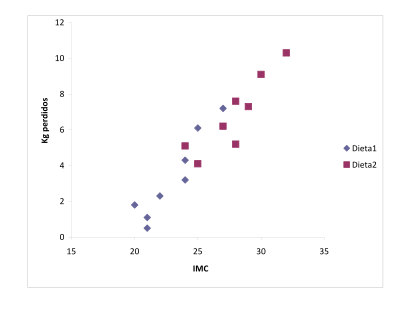
\includegraphics[scale=0.6]{anova_2_factores/img/covariable1}
\caption{Nube de puntos con covariable significativa pero no el factor}
\end{center}
\end{figure}

\item Si la nube de puntos se ajusta adecuadamente mediante varias rectas de pendiente nula, una por cada nivel del factor, entonces la
covariable no es significativa, pero sí el factor.

\item Si la nube de puntos se ajusta adecuadamente con rectas, una por cada nivel del factor, con igual pendiente no nula, y al menos una de
las rectas es diferente de todas las demás (al menos uno de los niveles aparece desplazado), entonces tanto la covariable como el factor
serían significativos a la hora de explicar la variable dependiente.

Por ejemplo, en la siguiente figura aparece el resultado de un experimento similar al ya comentado: Kg perdidos en función de la dieta y de
la covariable índice de masa corporal que no se ha controlado adecuadamente a la hora de hacer los grupos (el grupo de los que toman la
dieta 2 tiene mayor IMC de partida). A la vista de la gráfica incluso parece que hay diferencias significativas en el número de Kg perdidos
de tal forma que los de la dieta 2 haría perder más, pero todo es consecuencia de la covariable; eliminado su efecto, el número de Kg
perdidos por los individuos que toman la dieta 1 es mayor (eliminada la pendiente de la recta, los puntos de la dieta 1 quedarían por
arriba).

\begin{figure}[h!]
\begin{center}
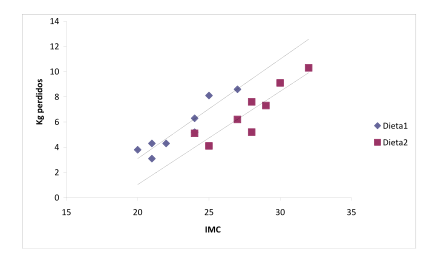
\includegraphics[scale=0.6]{anova_2_factores/img/covariable2}
\caption{Nube de puntos con covariable significativa y factor significativo}
\end{center}
\end{figure}

\item Si la nube de puntos se ajusta adecuadamente con diferentes rectas, una por cada nivel del factor, con pendientes no nulas pero
diferentes, entonces quiere decir que habría interacción entre covariable y factor y no debería plantearse un modelo de ANCOVA.
\end{itemize}


\section{Ejercicios resueltos}
\begin{enumerate}
\item En un estudio diseñado para analizar la influencia de un tipo de dieta y de un fármaco en el peso corporal perdido, expresado en Kg, se ha anotado el número de Kg perdidos en un grupo de personas al cabo de 3 meses de dieta y de tomar el fármaco, obteniendo los siguientes resultados (si algún individuo presenta un dato negativo significa que en lugar de perder Kg de peso los ha ganado):

\begin{center}

\begin{tabular}{|l|l|l|}
\cline{2-3}
\multicolumn{1}{c|}{} & \multicolumn{1}{c|}{Fármaco No} & \multicolumn{1}{c|}{Fármaco Sí} \\
\hline
\multicolumn{1}{|c|}{Dieta No} & \multicolumn{1}{c|}{1,5; 0,5; 0,0; -1,0; -1,0 } & \multicolumn{1}{c|}{6,5; 5,0; 7,0; 3,0; 4,5; 5,0} \\
\hline
\multicolumn{1}{|c|}{Dieta Sí} & \multicolumn{1}{c|}{3,5; 3,0; 4,0; 2,5; 2,0} & \multicolumn{1}{c|}{9,5; 8,0; 7,5; 7,0; 8,5; 7,5} \\
\hline
\end{tabular}

\end{center}

\begin{enumerate}

\item Crear la variables \textsf{Kilosperdidos}, \textsf{Dieta} y \textsf{Fármaco} e introducir los datos en PASW.

\begin{indicacion} {Al introducir los datos, tener en cuenta que tanto la \textsf{Dieta} como el \textsf{Fármaco} son variables cualitativas pero hay que introducirlas como numéricas. Posteriormente se puede asignar una etiqueta a los valores numéricos introducidos.}
\end{indicacion}

\item Realizar un ANOVA de dos vías con los datos e interpretar la tabla de ANOVA obtenida.

\begin{indicacion} {Para realizar el ANOVA propuesto, utilizar el menú \texttt{Analizar\flecha Modelo lineal general\flecha Univariante} y utilizar como \texttt{Variable dependiente} la variable \variable{Kilosperdidos} y como \texttt{Factores fijos} las variables \textsf{Dieta} y \textsf{Fármaco}. Por último pinchar en el botón \boton{Aceptar}.


Para la interpretación de la tabla de ANOVA, prestar especial atención a las siguientes líneas de la tabla:

\begin{enumerate}

\item Modelo Corregido: muestra si el modelo planteado para explicar el peso perdido en función de la dieta, el fármaco y la interacción de ambas es o no significativo globalmente, es decir, si es o no capaz de explicar un porcentaje considerable de la variabilidad de la variable dependiente. De hecho, en la parte baja de la tabla aparece el $R$ cuadrado del modelo (porcentaje de variabilidad explicado).
\item Dieta: muestra si la dieta resulta o no significativa para explicar la variabilidad del peso perdido.
\item Fármaco: muestra si el fármaco resulta o no significativo.
\item Dieta x Fármaco: muestra si la interacción de dieta y fármaco resulta o no significativa.


\end{enumerate}

Una conclusión muy importante a la luz de los resultados es que no hay una interacción significativa entre dieta y fármaco, es decir que el efecto del fármaco no dependerá de si una persona toma o no dieta, y a la inversa, que el efecto de la dieta no dependerá de si se toma o no fármaco.

}
\end{indicacion}

\item Mostrar el gráfico de medias correspondiente al anterior ANOVA. ¿Qué conclusiones cualitativas pueden sacarse del gráfico obtenido?

\begin{indicacion}{Para mostrar el gráfico de medias, que PASW llama gráfico de perfiles, repetir los pasos del anterior punto para realizar el ANOVA de dos vías pero antes de \texttt{Aceptar} pinchar en el botón \boton{Gráficos} y pasar al campo \campo{Eje horizontal}, por ejemplo, la variable \variable{Dieta}, y al campo \campo{Líneas separadas} la variable \variable{Fármaco}. Por último pinchar en el botón \boton{Añadir} y \texttt{Continuar}. Igualmente se podría obtener un gráfico de medias con la variable \variable{Fármaco} en el \texttt{Eje horizontal} y la \textsf{Dieta} en \texttt{Líneas separadas}.

Las conclusiones cualitativas: se observa claramente que no hay interacción (líneas paralelas), que los dos puntos del grupo de los que no hacen dieta están por debajo de los que sí que la hacen, lo cual hace sospechar que el factor dieta será significativo, e igualmente los dos puntos de los que no toman fármaco están por debajo de los que sí que lo toman, lo cual hace sospechar que el factor fármaco también será significativo.
}
\end{indicacion}

\item Calcular las medias y desviaciones típicas de los Kg perdidos en todos los grupos, tanto las reales como las estimadas por el modelo.

\begin{indicacion}{El procedimiento estadístico Modelo Lineal General Univariante de PASW, que es el que se está aplicando en este ejercicio, da la posibilidad de mostrar dos tipos diferentes de medias junto con sus desviaciones típicas:

\begin{itemize}
\item Las medias \emph{reales}, observadas o empíricas de cada uno de los grupos, teniendo en cuenta que en el problema se pueden calcular: la media global, las dos de los grupos que se forman con la variable dieta, las dos de los que se forman con la variable fármaco y las 4 que se forman con el cruce de dieta y fármaco.

\item Las medias que el programa llama \emph{estimadas}, que no son las reales sino las estimadas a partir de los parámetros del modelo que el programa genera cada vez que le pedimos que realice un ANOVA de varias vías. Internamente, para PASW un ANOVA de varias vías es un modelo de regresión multivariante en el que la variable dependiente se expresa como una función lineal de las diferentes variables independientes. Dicho modelo genera unos coeficientes de la combinación lineal que permiten estimar cuáles serían las medias de los diferentes grupos, con la ventaja de que estas medias llevarían eliminado el efecto que las demás variables, interacciones, o incluso covariables, podrían estar introduciendo. Por ejemplo, si se plantea calcular la media del grupo de los que siguen dieta y en dicho grupo da la casualidad de que prácticamente todos los individuos toman fármaco, su valor será más grande del que de verdad le correspondería si el grupo hubiese estado equilibrado (tantos que tomen fármaco como que no lo tomen). Esa media calculada eliminando la influencia del fármaco sería la estimada para el grupo de los que hacen dieta, y así cualquier otra. En realidad, siempre que aparezcan interacciones significativas, covariables significativas o los grupos que surjan de cruzar las variables no estén equilibrados (en nuestro problema hay dos grupos de 5 y dos de 6), se recomienda trabajar con las medias estimadas.


\end{itemize}

Para obtener un resumen estadístico con las medias y las desviaciones típicas reales: \texttt{Analizar\flecha Modelo lineal general\flecha Univariante}, en el botón \boton{Opciones}, en la parte de \texttt{Visualización} activar \texttt{Estadísticos descriptivos} y pinchar en el botón \boton{Continuar}. Las medias y desviaciones típicas se podrían obtener igualmente segmentando el archivo y aplicando los procedimientos oportunos de estadística descriptiva.

Para obtener un resumen estadístico con las medias estimadas: \texttt{Analizar\flecha Modelo lineal general\flecha Univariante}, y en el botón \boton{Opciones}, en la parte de \texttt{Medias marginales estimadas}, dentro de \texttt{Factores e interacciones de los factores} pasar toda la lista a \texttt{Mostrar las medias para} y pinchar en el botón \boton{Continuar}.

}
\end{indicacion}

\item Teniendo en cuenta que no hay interacción significativa, calcular los intervalos de confianza para las medias estimadas de los dos grupos que se forman con la variable dieta y el intervalo de confianza para la diferencia, todos con un 95\% de confianza. Igualmente con la variable fármaco.

\begin{indicacion}{Como la interacción no ha sido significativa, sólo cabe plantearse si hay diferencias significativas entre los que hacen dieta y los que no, y entre los que toman fármaco y los que no, pero en ningún caso habría que cruzar las variables (diferencias entre los que hacen dieta y los que no dentro del grupo de los que toman fármaco, diferencias entre los que hacen dieta y los que no dentro del grupo que no toma fármaco, diferencias entre los que toman fármaco y los que no dentro de los que hacen dieta o diferencias entre los que toman fármaco y los que no dentro de los que no hacen dieta). Además, ya sabemos que como tanto la dieta como el fármaco han resultado variables significativas, debe haber diferencias entre dieta sí y dieta no, y también entre fármaco sí y fármaco no, pero ahora se pide que se cuantifique el intervalo de confianza para la diferencia. Por otra parte, como los grupos no están equilibrados y además han salido significativas las dos variables, conviene trabajar con las medias estimadas en lugar de las reales. Afortunadamente, PASW junto con las medias estimadas también puede dar sus correspondientes intervalos de confianza tanto de forma individual como para las diferencias. Para ello: \texttt{Analizar\flecha Modelo lineal general\flecha Univariante}, y en el botón \boton{Opciones}, en la parte de \texttt{Medias marginales estimadas}, dentro de \texttt{Factores e interacciones de los factores} pasar \textsf{Dieta} y \textsf{Fármaco} a \texttt{Mostrar las medias para}, activar la casilla \texttt{Comparar los efectos principales} y como método de \texttt{Ajuste del intervalo de confianza} podemos escoger \texttt{Bonferroni} (en realidad, en este ejemplo no hay necesidad de ajustar los intervalos porque sólo hay dos categorías en cada variable, pero si hubiese tres o más, en lugar de una comparación se podrían realizar bastantes más y habría que controlar la posibilidad de un error de tipo I, por ejemplo, con el método de Bonferroni). Por último, pinchar en el botón \boton{Continuar}.

}
\end{indicacion}


\end{enumerate}


\item En un estudio diseñado para analizar la influencia de un tipo de dieta y de un fármaco en el peso corporal perdido, expresado en Kg, se ha anotado el número de Kg perdidos en un grupo de personas al cabo de 3 meses de dieta y de tomar el fármaco, obteniendo los siguientes resultados (si algún individuo presenta un dato negativo significa que en lugar de perder Kg de peso los ha ganado):

\begin{center}

\begin{tabular}{|l|l|l|}
\cline{2-3}
\multicolumn{1}{c|}{} & \multicolumn{1}{c|}{Fármaco No} & \multicolumn{1}{c|}{Fármaco Sí} \\
\hline
\multicolumn{1}{|c|}{Dieta No} & \multicolumn{1}{c|}{1,5; 0,5; 0,0; -1,0; -1,0 } & \multicolumn{1}{c|}{6,5; 5,0; 7,0; 3,0; 4,5; 5,0} \\
\hline
\multicolumn{1}{|c|}{Dieta Sí} & \multicolumn{1}{c|}{3,5; 3,0; 4,0; 2,5; 2,0} & \multicolumn{1}{c|}{12,5; 12,0; 11,5; 13,5; 12,5; 10,0} \\
\hline
\end{tabular}

\end{center}

\begin{enumerate}

\item Crear la variables \textsf{Kilosperdidos}, \textsf{Dieta} y \textsf{Fármaco} e introducir los datos en PASW.

\begin{indicacion}{Seguir el mismo proceso del apartado a del ejercicio anterior.

}
\end{indicacion}

\item Realizar un ANOVA de dos vías con los datos e interpretar la tabla de ANOVA obtenida. ¿Hay interacción significativa? ¿Cómo se interpretaría?

\begin{indicacion}{Para obtener la tabla de ANOVA, seguir el mismo proceso del apartado b del ejercicio anterior.

Sí que hay interacción significativa y eso implica que no hay la misma diferencia en Kg perdidos entre los que hacen dieta y los que no si consideramos el grupo de los que no toman fármaco que si consideramos el grupo de los que sí que lo toman.

}
\end{indicacion}

\item Mostrar el gráfico de medias correspondiente al anterior ANOVA. ¿Qué conclusiones cualitativas pueden sacarse del gráfico obtenido?

\begin{indicacion}{Para obtener el gráfico de medias, seguir el mismo proceso del apartado c del ejercicio anterior.

La interpretación del gráfico es que ahora se ve claramente que además de ser la dieta y el fármaco significativos, también lo es la interacción (las líneas que unen las medias tienen pendientes muy diferentes).

}
\end{indicacion}

\item ¿Entre qué medias sería adecuado buscar diferencias significativas en este problema? Calcular las medias, junto con sus intervalos de confianza con un 95\%, tanto de las medias como de sus diferencias.

\begin{indicacion}{Por tratarse de un problema en el que hay interacción entre dieta y fármaco, se debería ver si hay diferencias entre dieta sí y dieta no en el grupo de los que toman fármaco, y entre dieta sí y dieta no en el grupo de los que no lo toman. Igualmente se podría analizar la diferencia entre fármaco sí y fármaco no en el grupo de los que hacen dieta, y entre fármaco sí y fármaco no en el grupo de los que no la hacen. Trabajando con las medias estimadas: \texttt{Analizar\flecha Modelo lineal general\flecha Univariante}, y en el botón \boton{Opciones}, en la parte de \texttt{Medias marginales estimadas}, dentro de \texttt{Factores e interacciones de los factores} pasar toda la lista a \texttt{Mostrar las medias para}, activar la casilla \texttt{Comparar los efectos principales} y escoger como \texttt{Método de ajuste del intervalo} de confianza \texttt{Bonferroni}.

Pero se puede observar en el resultado que aparece que PASW, por defecto, no realiza nada más que las comparaciones en los factores principales, que por otra parte no son las que interesan en este problema ya que hay interacción. Para que realice las comparaciones debidas a la interacción no queda más remedio que obligar al programa a realizarlas mediante comandos. Para ello, hay que generar el \emph{Archivo de Sintaxis} (conjunto de órdenes) del procedimiento estadístico con el que se está trabajando y añadirle los comandos adecuados.

Para generar el archivo de sintaxis, en lugar de pinchar en el botón \boton{Aceptar} al final de todo el proceso, se pincha en el botón \boton{Pegar}. Eso hace que se abra el Editor de Sintaxis, con un conjunto de comandos que son los que dan las órdenes adecuadas al programa para que ejecute los procesos pedidos. Para que realice la comparación dentro de los grupos generados mediante el cruce de variables, hay que retocar la línea en la que muestra sus medias, /EMMEANS=TABLES(Dieta*Fármaco), que debe incluir: COMPARE(Fármaco) ADJ(BONFERRONI). Su aspecto final debe ser:

/EMMEANS=TABLES(Dieta*Fármaco) COMPARE(Fármaco) ADJ(BONFERRONI)

Y también hay que añadir una línea más justo a continuación de la anterior:

/EMMEANS=TABLES(Fármaco*Dieta) COMPARE(Dieta) ADJ(BONFERRONI)


Una vez hechos los cambios, se marca todo el texto arrastrando el ratón y se ejecutan los comandos seleccionados con el menú \texttt{Ejecutar\flecha Selección}. Con ello, se obtienen todas las comparaciones junto con sus intervalos de confianza.


}
\end{indicacion}

\end{enumerate}

\item Se ha realizado un experimento que consiste en que se ha anotado el tiempo, en días, que han tardado en contestar correctamente a un cuestionario 30 personas, 15 hombres y 15 mujeres, distribuidos en grupos que han seguido tres métodos diferentes de aprendizaje de la materia del cuestionario. Los resultados aparecen en la siguiente tabla:

\begin{center}

\begin{tabular}{|l|l|l|l|}
\cline{2-4}
\multicolumn{1}{c|}{} & \multicolumn{1}{c|}{Método a } & \multicolumn{1}{c|}{Método b} & \multicolumn{1}{c|}{Método c} \\
\hline
\multicolumn{1}{|c|}{Hombre} & \multicolumn{1}{c|}{15, 16, 18, 19, 14} & \multicolumn{1}{c|}{25, 27, 28, 23, 29} & \multicolumn{1}{c|}{21, 22, 18, 17, 20} \\
\hline
\multicolumn{1}{|c|}{Mujer} & \multicolumn{1}{c|}{24, 27, 29, 25, 23} & \multicolumn{1}{c|}{17, 15, 13, 16, 18} & \multicolumn{1}{c|}{20, 19, 22, 17, 23} \\
\hline
\end{tabular}

\end{center}

\begin{enumerate}

\item Crear las variables Sexo, Método y Días, e introducir los datos.

\item Generar la tabla de ANOVA de dos vías con interacción e interpretar los resultados.

\begin{indicacion}{Utilizar el menú \texttt{Analizar\flecha Modelo lineal general\flecha Univariante} y utilizar como \texttt{Variable dependiente} la variable \variable{Días} y como \texttt{Factores fijos} las variables \textsf{Sexo} y \textsf{Método}. Por último pinchar en el botón \boton{Aceptar}.

Interpretación: no hay diferencias significativas asociadas al sexo ni al método. Sin embargo sí que hay interacción, es decir la diferencia en el tiempo de respuesta entre hombres y mujeres depende del método seguido, e igualmente las diferencias entre los tiempos de respuesta según los diferentes métodos dependen del sexo.

}
\end{indicacion}


\item Generar dos gráficos de medias: un primero en el que en el eje horizontal aparezca el Método y con líneas distintas según Sexo, y un segundo en el que en el eje horizontal aparezca el Sexo y líneas distintas para el Método. ¿Qué se puede decir de la interacción de las variables?

\begin{indicacion}{Repetir los pasos del anterior punto para realizar el ANOVA de dos vías pero antes de \texttt{Aceptar} pinchar en el botón \boton{Gráficos} y pasar al campo \campo{Eje horizontal} la variable \variable{Método}, y al campo \campo{Líneas separadas} la variable \variable{Sexo} y se pincha en el botón \boton{Añadir}. Para el siguiente gráfico, sin necesidad de repetir todo el proceso, se pasa al \texttt{Eje horizontal} la variable \variable{Sexo} y al campo \campo{Líneas separadas} la variable \variable{Método} y se pincha en el botón \boton{Añadir}. Posteriormente se pincha en \texttt{Continuar} y \texttt{Aceptar}.

Interpretación: es evidente que las líneas se cruzan, lo cual indica que hay interacción.

}
\end{indicacion}

\item Calcular las medias estimadas y sus correspondientes intervalos de confianza, además de analizar entre qué medias hay diferencias y sus correspondientes intervalos de confianza para la diferencia. Trabajar con un 95\% de confianza.

\begin{indicacion}{De nuevo, las medias que de verdad interesan son las que surgen del cruce de los dos factores. Para poder ver la diferencia entre hombre y mujeres, tanto en el método a como el b y el c; y para poder ver la diferencia entre los métodos a y b, a y c y b y c, tanto en el grupo de hombres como en el de mujeres, acudimos de nuevo a las medias estimadas y hacemos las comparativas: \texttt{Analizar\flecha Modelo lineal general\flecha Univariante}, y en el botón \boton{Opciones}, en la parte de \texttt{Medias marginales estimadas}, dentro de \texttt{Factores e interacciones de los factores} pasar toda la lista a \texttt{Mostrar las medias para}, activar la casilla \texttt{Comparar los efectos principales} y escoger como \texttt{Método de ajuste del intervalo} de confianza \texttt{Bonferroni}. Posteriormente se genera el archivo de sintaxis, pinchando en el botón \boton{Pegar} en lugar de \texttt{Aceptar}. Eso hace que se abra el Editor de Sintaxis, donde, para que realice la comparación dentro de los grupos generados mediante el cruce de variables, hay que retocar la línea en la que muestra sus medias, /EMMEANS=TABLES(Sexo*Método), que debe incluir: COMPARE(Método) ADJ(BONFERRONI). Su aspecto final debe ser:

/EMMEANS=TABLES(Sexo*Método) COMPARE(Método) ADJ(BONFERRONI)

Y también hay que añadir una línea más justo a continuación de la anterior:

/EMMEANS=TABLES(Método*Sexo) COMPARE(Sexo) ADJ(BONFERRONI)


Una vez hechos los cambios, se marca todo el texto arrastrando el ratón y se ejecutan los comandos seleccionados con el menú \texttt{Ejecutar\flecha Selección}. Con ello, se obtienen todas las comparaciones junto con sus intervalos de confianza.



}
\end{indicacion}

\end{enumerate}

\item Se ha realizado un experimento para comprobar si los Kg perdidos por un grupo de personas dependen o no de la dieta utilizada durante 3 meses. Para ello se ha trabajado con dos dietas diferentes y se ha anotado el número de Kg perdidos y el índice de masa corporal (IMC) de los individuos. Los resultados aparecen en la siguiente tabla:

\begin{center}

\begin{tabular}{|l|l|l|}
\hline
\multicolumn{1}{|c|}{Kg perdidos} & \multicolumn{1}{c|}{Dieta} & \multicolumn{1}{c|}{IMC} \\
\hline
\multicolumn{1}{|c|}{4,3} & \multicolumn{1}{c|}{1} & \multicolumn{1}{c|}{24} \\
\hline
\multicolumn{1}{|c|}{1,8} & \multicolumn{1}{c|}{1} & \multicolumn{1}{c|}{20} \\
\hline
\multicolumn{1}{|c|}{6,1} & \multicolumn{1}{c|}{1} & \multicolumn{1}{c|}{25} \\
\hline
\multicolumn{1}{|c|}{2,3} & \multicolumn{1}{c|}{1} & \multicolumn{1}{c|}{22} \\
\hline
\multicolumn{1}{|c|}{1,1} & \multicolumn{1}{c|}{1} & \multicolumn{1}{c|}{21} \\
\hline
\multicolumn{1}{|c|}{0,5} & \multicolumn{1}{c|}{1} & \multicolumn{1}{c|}{21} \\
\hline
\multicolumn{1}{|c|}{7,2} & \multicolumn{1}{c|}{1} & \multicolumn{1}{c|}{27} \\
\hline
\multicolumn{1}{|c|}{3,2} & \multicolumn{1}{c|}{1} & \multicolumn{1}{c|}{24} \\
\hline
\multicolumn{1}{|c|}{9,1} & \multicolumn{1}{c|}{2} & \multicolumn{1}{c|}{30} \\
\hline
\multicolumn{1}{|c|}{5,2} & \multicolumn{1}{c|}{2} & \multicolumn{1}{c|}{28} \\
\hline
\multicolumn{1}{|c|}{7,3} & \multicolumn{1}{c|}{2} & \multicolumn{1}{c|}{29} \\
\hline
\multicolumn{1}{|c|}{10,3} & \multicolumn{1}{c|}{2} & \multicolumn{1}{c|}{32} \\
\hline
\multicolumn{1}{|c|}{5,1} & \multicolumn{1}{c|}{2} & \multicolumn{1}{c|}{24} \\
\hline
\multicolumn{1}{|c|}{7,6} & \multicolumn{1}{c|}{2} & \multicolumn{1}{c|}{28} \\
\hline
\multicolumn{1}{|c|}{6,2} & \multicolumn{1}{c|}{2} & \multicolumn{1}{c|}{27} \\
\hline
\multicolumn{1}{|c|}{4,1} & \multicolumn{1}{c|}{2} & \multicolumn{1}{c|}{25} \\
\hline
\end{tabular}

\end{center}

\begin{enumerate}

\item Crear las variables Kgperdidos, Dieta y IMC e introducir los datos de la tabla.


\item Sin tener en cuenta la variable IMC, ¿se puede considerar que la variable dieta influye significativamente en la cantidad de Kg perdidos?

\begin{indicacion}{Como en este caso sólo hay dos categorías de la variable dieta, se puede hacer la comparación mediante una T de Student de datos independientes: \texttt{Analizar\flecha Comparar Media\flecha Prueba T para muestras independientes}, la \texttt{Variable para contrastar} son los \textsf{Kgperdidos} y la \texttt{Variable de agrupación} la \textsf{Dieta}, en la que habrá que definir adecuadamente los grupos. A la vista de los resultados, con un 95\% de confianza se puede afirmar que la dieta influye en la cantidad de Kg perdidos.

La T de Student de datos independientes tiene la ventaja de que da directamente el intervalo para la diferencia. No obstante, como la pregunta es si la dieta influye significativamente en la cantidad de Kg perdidos y no se piden los intervalos de confianza, para realizar el contraste de igualdad de las dos medias también se puede hacer un ANOVA de una vía mediante: \texttt{Analizar\flecha Comparar medias\flecha ANOVA de un factor}, o incluso a través del procedimiento \texttt{Analizar\flecha Modelo lineal general\flecha Univariante}, que en principio está diseñado para realizar ANOVAS de varias vías pero también se puede utilizar para un único factor.


}
\end{indicacion}

\item Representar la nube de puntos de la cantidad de Kg perdidos en función del IMC coloreando los puntos según la Dieta seguida. A la vista del gráfico, ¿la cantidad de Kg perdidos depende de la dieta o más bien del IMC del individuo?

\begin{indicacion}{Como cualquier otro diagrama de dispersión, se puede generar mediante: \texttt{Gráficos\flecha Cuadros de diálogo antiguos\flecha Dispersión/Puntos}, escoger \texttt{Dispersión simple}, pinchar en \texttt{Definir}, escoger como \texttt{Eje Y} la variable \variable{Kgperdidos}, como \texttt{Eje X} el \textsf{IMC} y \texttt{Establecer marcas por} la variable \variable{Dieta}.

Interpretación: se ve claramente que todos los puntos, ya sean los de la dieta 1 o la 2, aparecen en una nube que se puede ajustar con una única recta de pendiente no nula que marca la influencia de la covariable IMC, pero eliminado el efecto del IMC, es decir, si arrastramos los puntos hacia abajo para dejar la recta con pendiente 0, todos los puntos quedarían a una altura similar, por lo que no habría influencia de la dieta.


}
\end{indicacion}

\item Realizar un ANCOVA con la variable dependiente Kgperdidos, el factor dieta y la covariable IMC. Interpretar los resultados obtenidos.

\begin{indicacion}{Para generar la tabla del ANOVA con la covariable añadida, \texttt{Analizar\flecha Modelo lineal general\flecha Univariantes}, seleccionar como \texttt{Variable dependiente} \textsf{Kgperdidos}, como \texttt{Factores Fijos} la \textsf{Dieta} y como \texttt{Covariables} el \texttt{IMC}.

Interpretación: El número de Kg perdidos no depende significativamente de la dieta y es simplemente la covariable la que hace que parezca que los individuos que siguen la dieta 1 pierdan más Kg que los que siguen la dieta 2.

}
\end{indicacion}

\item Mostrar las medias reales y las estimadas. ¿Hay diferencias estadísticamente significativas entre las estimadas?

\begin{indicacion}{

Para mostrar las medias reales, se pueden seguir múltiples caminos dentro del programa; entre otros, repetir los pasos dados en el punto anterior, pinchar en el botón \boton{Opciones} y en la parte \texttt{Visualización} escoger \texttt{Estadísticos descriptivos}.

Para mostrar las medias estimadas (en las que se ha eliminado el efecto de la covariable) seguir los mismos pasos pero, después de pinchar en el botón \boton{Opciones}, ir a la parte de \texttt{Medias marginales estimadas}, escoger en \texttt{Factores e interacciones de los factores} tanto \textsf{OVERALL} como \textsf{Dieta} y pasar al campo \campo{Mostrar las medias para}. Por último, activar \texttt{Comparar los efectos principales} y como método de \texttt{Ajuste del intervalo de confianza} vale cualquiera porque en este caso sólo hay dos niveles (habitualmente se puede escoger \texttt{Bonferroni}).

Interpretación: Las medias muestrales reales de los dos grupos y sus correspondiente estimadas son claramente diferentes. Al eliminar el efecto de la covariable incluso la media muestral estimada de los que toman la dieta 2 es menor que la del grupo 1 cuando en las reales era justo al revés. No obstante, entre las estimadas no hay diferencias estadísticamente significativas (el intervalo para la diferencia contiene al 0) con un 95\% de confianza.

}
\end{indicacion}

\item Repetir el ANCOVA con la comparación de medias, tanto reales como estimadas, pero suponiendo que los Kg perdidos por los que han seguido la dieta 1 son: 6,3; 3,8; 8,1; 4,3; 3,1; 4,3; 8,6; 5,2. Obtener también el diagrama de dispersión con el código de colores según dieta.

\begin{indicacion}{Seguir exactamente los mismos pasos que en los puntos anteriores del ejercicio.
}

\end{indicacion}

\end{enumerate}

\item Se desea comparar la rapidez con la que aparece el efecto de tres nuevos agentes repigmentadores: A, B y C. Con esta intención, se aplican de manera tópica dosis equivalentes de los tres repigmentadores en zonas de la piel con pérdida total de pigmentación en los mismos ocho pacientes con vitíligo. A continuación, se recoge el tiempo, en días, que tardan en aparecer los primeros signos de repigmentación:


\begin{center}
\begin{tabular}{|l|l|l|}
\hline
\multicolumn{1}{|c|}{A} & \multicolumn{1}{c|}{B} & \multicolumn{1}{c|}{C} \\
\hline
\multicolumn{1}{|c|}{19} & \multicolumn{1}{c|}{3} & \multicolumn{1}{c|}{31} \\
\hline
\multicolumn{1}{|c|}{11} & \multicolumn{1}{c|}{2} & \multicolumn{1}{c|}{9} \\
\hline
\multicolumn{1}{|c|}{7} & \multicolumn{1}{c|}{4} & \multicolumn{1}{c|}{16} \\
\hline
\multicolumn{1}{|c|}{4} & \multicolumn{1}{c|}{1} & \multicolumn{1}{c|}{6} \\
\hline
\multicolumn{1}{|c|}{3} & \multicolumn{1}{c|}{2} & \multicolumn{1}{c|}{8} \\
\hline
\multicolumn{1}{|c|}{5} & \multicolumn{1}{c|}{7} & \multicolumn{1}{c|}{18} \\
\hline
\multicolumn{1}{|c|}{7} & \multicolumn{1}{c|}{1} & \multicolumn{1}{c|}{5} \\
\hline
\multicolumn{1}{|c|}{4} & \multicolumn{1}{c|}{3} & \multicolumn{1}{c|}{9} \\
\hline
\end{tabular}

\end{center}


\begin{enumerate}

\item Crear las variable A, B y C e introducir los datos en PASW conforme se dan en la tabla anterior (cada individuo en una fila y las 3 medidas diferentes en 3 variables).

\item Realizar un ANOVA de medidas repetidas e interpretar el resultado obtenido.

\begin{indicacion}{PASW dispone de un procedimiento estadístico específico para la realización de ANOVAS de medidas repetidas cuando los datos se introducen en el formato clásico de una fila por individuo y una variable por cada una de las medidas repetidas. Para acceder al procedimiento: \texttt{Analizar\flecha Modelo lineal general\flecha Medidas repetidas}. En el campo \campo{Nombre del factor intra-sujetos} se da nombre al factor que contendrá las medidas repetidas, que en este caso son tiempos expresados en días, por lo que se puede llamar \textsf{Tiempo}. En el campo \campo{Número de niveles} hay que poner el número de medidas repetidas, es decir, el número de niveles del factor \textsf{Tiempo} que son 3. Posteriormente se pincha en el botón \boton{Añadir} para añadir el factor a la lista de factores intra-sujetos (permite trabajar con varios) y en el botón \boton{Definir} para dar las variables que forman los niveles del factor y en el campo \campo{Variables intra-sujetos} introducimos \textsf{A}, \textsf{B} y \texttt{C}. Antes de pinchar en el botón \boton{Aceptar} para obtener el ANOVA de medidas repetidas, se puede observar que el procedimiento estadístico permite incluir en el análisis factores inter-sujetos (que más bien son factores inter-grupos), por ejemplo el sexo, y covariables, por ejemplo la edad; por lo tanto, este procedimiento permite realizar el ANOVA más completo posible: varios factores intra-sujetos, varios factores inter-sujetos y varias covariables. Por último, se pincha en \texttt{Aceptar} y se obtiene el resultado del ANOVA.

Interpretación:

El resultado obtenido contiene varias tablas pero, esencialmente, las más importantes son:

\begin{itemize}

\item La tabla que el programa llama \texttt{Prueba de los efectos intra-sujetos}, que en su primera línea (Esfericidad Asumida) da el $p$-valor del contraste de igualdad de medias de todos los niveles del factor intra-sujetos. Esta tabla presentaría más líneas como la comentada si se hubiesen añadido más factores intra-sujeto al estudio, y también la interacción entre los factores intra-sujeto con los factores inter-sujetos y las covariables, si es que los hubiese en el estudio considerado.

\item La tabla que el programa llama \texttt{Prueba de los efectos inter-sujetos}, que en este caso no tiene ninguna línea importante ya que no se han añadido al estudio factores inter-sujeto ni covariables. Mostraría el p-valor de todos los factores inter-sujetos, de las covariables y de la interacción entre de los factores inter-sujetos entre sí.

\item También muestra una tabla de Prueba de esfericidad de Mauchly que es la prueba con la que se contrastan los supuestos del modelo de ANOVA de medidas repetidas. Si el p-valor de la prueba sale mayor que el nivel de significación entonces no se puede rechazar la hipótesis nula de esfericidad de los datos (distribuciones normales en todos los grupos con homogeneidad de varianzas). Si se rechaza la esfericidad mejor que en el ANOVA de medidas repetidas convendría fijarse en el resultado de los Contrastes Multivariados que aparecen en otra tabla y que no necesitan esfericidad para poder ser calculados.

\end{itemize}

En el caso concreto del problema, el factor intra-sujetos definido, el tiempo, sí que resulta significativo, por lo que al menos una de las medidas repetidas tiene una media diferente de las demás.

}
\end{indicacion}

\item ¿Entre qué medidas del factor intra-sujetos se dan diferencias estadísticamente significativas?

\begin{indicacion}{Después de \texttt{Analizar\flecha Modelo lineal general\flecha Medidas repetidas} y definir el factor intra-sujetos, \textsf{Tiempo}, con 3 niveles, dentro del cuadro de diálogo que aparece (Medidas Repetidas), pinchando en el botón \boton{Opciones}, en la parte de \texttt{Medias marginales estimadas} ir a la lista de \texttt{Factores e interacciones de los factores} y escoger \textsf{OVERALL} y \textsf{Tiempo} y pasarlas a \texttt{Mostrar las medias para}. Después, activar la casilla \texttt{Comparar los efectos principales} y como \texttt{Ajuste del intervalo de confianza} utilizar \texttt{Bonferroni}.

Interpretación: en la tabla de Comparaciones por pares que aparece se ve que hay diferencias significativas entre los tiempos 2 y 3, es decir entre el tiempo en que comienzan a aparecer signos de repigmentación con el agente B y el C.



}
\end{indicacion}


\item Realizar el mismo ANOVA de medidas repetidas pero introduciendo los datos como se darían en un ANOVA de dos vías con la variable cuantitativa dependiente Tiempo y los factores cualitativos Repigmentador e Individuo.

\begin{indicacion}{Si se pretenden hacer un ANOVA de medidas repetidas como si fuese un ANOVA de dos vías sin interacción, lo primero es introducir los datos de tal forma que cada individuo ocupa tantas filas como medidas repetidas se han dado. Para ello se genera una variable Tiempo que contiene los 24 tiempos, una variable Repigmentador numérica con valores 1, 2 y 3 (a los que se pueden asignar las etiquetas de valor A, B y C), y una variable Individuo con valores desde el 1 al 8 repetidos 3 veces:

\begin{center}

\begin{tabular}{|l|l|l|}
\hline
\multicolumn{1}{|c|}{Tiempo} & \multicolumn{1}{c|}{Repigmentador} & \multicolumn{1}{c|}{Individuo} \\
\hline
\multicolumn{1}{|c|}{19} & \multicolumn{1}{c|}{1} & \multicolumn{1}{c|}{1} \\
\hline
\multicolumn{1}{|c|}{11} & \multicolumn{1}{c|}{1} & \multicolumn{1}{c|}{2} \\
\hline
\multicolumn{1}{|c|}{...} & \multicolumn{1}{c|}{...} & \multicolumn{1}{c|}{...} \\
\hline
\multicolumn{1}{|c|}{4} & \multicolumn{1}{c|}{1} & \multicolumn{1}{c|}{8} \\
\hline
\multicolumn{1}{|c|}{3} & \multicolumn{1}{c|}{2} & \multicolumn{1}{c|}{1} \\
\hline
\multicolumn{1}{|c|}{2} & \multicolumn{1}{c|}{2} & \multicolumn{1}{c|}{2} \\
\hline
\multicolumn{1}{|c|}{...} & \multicolumn{1}{c|}{...} & \multicolumn{1}{c|}{...} \\
\hline
\multicolumn{1}{|c|}{3} & \multicolumn{1}{c|}{2} & \multicolumn{1}{c|}{8} \\
\hline
\multicolumn{1}{|c|}{31} & \multicolumn{1}{c|}{3} & \multicolumn{1}{c|}{1} \\
\hline
\multicolumn{1}{|c|}{9} & \multicolumn{1}{c|}{3} & \multicolumn{1}{c|}{2} \\
\hline
\multicolumn{1}{|c|}{...} & \multicolumn{1}{c|}{...} & \multicolumn{1}{c|}{...} \\
\hline
\multicolumn{1}{|c|}{9} & \multicolumn{1}{c|}{3} & \multicolumn{1}{c|}{8} \\
\hline
\end{tabular}

\end{center}

Una vez introducidos los datos en el formato adecuado, el ANOVA de dos vías sin interacción se hace con: \texttt{Analizar\flecha Modelo lineal general\flecha Univariante}; escoger como \texttt{Variable dependiente} el \textsf{Tiempo} y como \texttt{Factores fijos} \textsf{Repigmentador} e \textsf{Individuo}, y pinchando en el botón \boton{Modelo} escoger en \texttt{Especificar modelo} el tipo \texttt{Personalizado}, en \texttt{Construir términos} escoger como \texttt{Tipo} la opción \opcion{Efectos principales }(no debe haber interacción) y pasar \textsf{Repigmentador} e \textsf{Individuo} al campo \campo{Modelo}. Por último pinchar en los botones \texttt{Continuar} y \texttt{Aceptar}. Con ello se obtiene la tabla del ANOVA en la que se puede ver que el $p$-valor obtenido para el factor inter-sujetos Repigmentador es el mismo que el obtenido para el factor intra-sujetos del ANOVA de medidas repetidas.

}
\end{indicacion}

\end{enumerate}

\item En un estudio sobre la memoria realizado con 12 personas se ha registrado el número de aciertos en una secuencia de números en tres periodos temporales distintos: tras una hora de entrenamiento, tras un día y tras una semana. De las 12 personas, 6 han seguido un método de entrenamiento y las otras 6 otro diferente. Además, se piensa que la edad de los individuos puede influir en el resultado y temiendo que los dos grupos de 6 individuos no tengan una distribución homogénea de edades, la misma se incluye como covariable. Los datos obtenidos han sido:

\begin{center}

  \begin{tabular}{|l|l|l|l|l|}
\cline{2-5}
\multicolumn{1}{c|}{} & \multicolumn{1}{c|}{Hora} & \multicolumn{1}{c|}{Día} & \multicolumn{1}{c|}{Semana} & \multicolumn{1}{c|}{Edad} \\
\hline
\multicolumn{1}{|c|}{Método 1} & \multicolumn{1}{c|}{4} & \multicolumn{1}{c|}{5} & \multicolumn{1}{c|}{7} & \multicolumn{1}{c|}{43} \\
\cline{2-5}
\multicolumn{1}{|c|}{} & \multicolumn{1}{c|}{6} & \multicolumn{1}{c|}{8} & \multicolumn{1}{c|}{10} & \multicolumn{1}{c|}{48} \\
\cline{2-5}
\multicolumn{1}{|c|}{} & \multicolumn{1}{c|}{1} & \multicolumn{1}{c|}{6} & \multicolumn{1}{c|}{5} & \multicolumn{1}{c|}{56} \\
\cline{2-5}
\multicolumn{1}{|c|}{} & \multicolumn{1}{c|}{2} & \multicolumn{1}{c|}{10} & \multicolumn{1}{c|}{12} & \multicolumn{1}{c|}{36} \\
\cline{2-5}
\multicolumn{1}{|c|}{} & \multicolumn{1}{c|}{5} & \multicolumn{1}{c|}{10} & \multicolumn{1}{c|}{10} & \multicolumn{1}{c|}{35} \\
\cline{2-5}
\multicolumn{1}{|c|}{} & \multicolumn{1}{c|}{1} & \multicolumn{1}{c|}{7} & \multicolumn{1}{c|}{8} & \multicolumn{1}{c|}{51} \\
\hline
\multicolumn{1}{|c|}{Método 2} & \multicolumn{1}{c|}{1} & \multicolumn{1}{c|}{2} & \multicolumn{1}{c|}{4} & \multicolumn{1}{c|}{59} \\
\cline{2-5}
\multicolumn{1}{|c|}{} & \multicolumn{1}{c|}{3} & \multicolumn{1}{c|}{6} & \multicolumn{1}{c|}{6} & \multicolumn{1}{c|}{46} \\
\cline{2-5}
\multicolumn{1}{|c|}{} & \multicolumn{1}{c|}{3} & \multicolumn{1}{c|}{5} & \multicolumn{1}{c|}{4} & \multicolumn{1}{c|}{53} \\
\cline{2-5}
\multicolumn{1}{|c|}{} & \multicolumn{1}{c|}{1} & \multicolumn{1}{c|}{4} & \multicolumn{1}{c|}{7} & \multicolumn{1}{c|}{45} \\
\cline{2-5}
\multicolumn{1}{|c|}{} & \multicolumn{1}{c|}{5} & \multicolumn{1}{c|}{6} & \multicolumn{1}{c|}{5} & \multicolumn{1}{c|}{49} \\
\cline{2-5}
\multicolumn{1}{|c|}{} & \multicolumn{1}{c|}{2} & \multicolumn{1}{c|}{8} & \multicolumn{1}{c|}{7} & \multicolumn{1}{c|}{39} \\
\hline
\end{tabular}

\end{center}

\begin{enumerate}

\item Crear las variables Método (se introduce como numérica pero es cualitativa, aunque se le pueden asignar etiquetas de valor), Hora, Día, Semana y Edad e introducir los datos en PASW.



\item Realizar un ANOVA de medidas repetidas pero teniendo en cuenta el factor inter-sujetos Método y también la covariable Edad. Interpretar el resultado obtenido.

\begin{indicacion}{Para obtener las tablas ANOVA de medidas repetidas: \texttt{Analizar\flecha Modelo lineal general\flecha Medidas repetidas}. En el campo \campo{Nombre del factor intra-sujetos} se puede poner cualquiera, por ejemplo aprovechando las iniciales de hora, día y semana que son los momentos en los que se realizan las diferentes medidas se puede llamar \textsf{Hds}; su \texttt{Número de niveles} es 3; se pincha en el botón \boton{Añadir} y luego en \texttt{Definir} para escoger \texttt{Variables intra-sujetos} que son \textsf{Hora}, \textsf{Día} y \textsf{Semana}; en \texttt{Factores inter-sujetos} la variable \variable{Método} y en \texttt{Covariables} la \textsf{Edad}. Por último, se pincha en \texttt{Aceptar}.


Interpretación de las tablas:

Mirando en la tabla de Pruebas de efectos intra-sujetos se ve que el factor Hds, con esfericidad asumida, ha resultado significativo. Es decir, hay una evolución en el número de aciertos según el tiempo; en definitiva, hay alguna media (ya sea la de Hora, Día o Semana) cuya diferencia con alguna de las demás es significativa. En la misma tabla se observa que no hay interacción significativa entre Hds y Edad ni entre Hds y Método. Por lo tanto esa evolución significativa, esa diferencia en el número de aciertos entre los niveles del factor intra no depende ni del Método ni de la Edad.

Mirando en la tabla de Pruebas de efectos inter-sujetos se ve que tanto la Edad como el Método han resultado significativos. Es decir, el número de aciertos tiene una correlación no nula con la Edad, y además también hay diferencias entre el número de aciertos de los que han seguido un método de aprendizaje y los que han seguido otro.


}
\end{indicacion}

\item ¿Entre qué medias estimadas hay diferencias significativas?

\begin{indicacion}{Para ver entre qué medias estimadas hay diferencias significativas, después de definir los factores intra-sujetos, inter-sujetos y las covariables, se pincha en el botón \boton{Opciones}, en \texttt{Medias marginales estimadas} ir a \texttt{Factores e interacciones de los factores} y escoger \textsf{Método} y \textsf{Hds} (también se puede escoger la global, \textsf{OVERALL}, y las que surgen de la interacción, pero la interacción no ha resultado significativa) y pasarlas a \texttt{Mostrar las medias para}. Posteriormente activar \texttt{Comparar los efectos principales} y como método de \texttt{Ajuste del intervalo de confianza} escoger \texttt{Bonferroni}.

Interpretación: Al analizar la comparativa de medias estimadas se observa que el Método 1 logra una cantidad significativamente mayor que el 2. Además también hay diferencias entre los aciertos que se obtienen entre una hora de entrenamiento y al cabo de un día y una semana, pero no hay diferencia significativa entre los resultados al cabo de un día y al cabo de una semana.

}
\end{indicacion}

\item Obtener todos los gráficos de medias estimadas posibles en el problema.

\begin{indicacion}{En el problema se pueden obtener hasta 4 gráficos de medias:

\begin{itemize}

\item El correspondiente a las medias estimadas en ambos métodos de entrenamiento. Con este gráfico se puede comprobar cualitativamente que hay diferencias entre los dos métodos.

\item El correspondiente a las medias estimadas de Hds (Horas, Días, Semanas). Con este gráfico se puede comprobar cualitativamente que hay diferencias entre las medias de las 3 medidas relacionadas diferentes.

\item La medias que surgen del cruce de Método con Hds, con el Método en el Eje X y líneas diferentes para Hds. Con este gráfico se puede comprobar cualitativamente que no hay interacción, es decir que las diferencias dentro del método 1 son parecidas a las que se dan en el método 2.

\item Las medias que surgen del cruce de Método con Hds, con el Hds en el Eje X y línea diferentes para el Método. Con este gráfico se puede comprobar cualitativamente que no hay interacción, es decir que las diferencias entre los dos métodos son parecidas al cabo de una hora, al cabo de un día y al cabo de una semana.


\end{itemize}

Para obtener los gráficos, después de definir los factores intra-sujetos, inter-sujetos y las covariables, se pincha en el botón \boton{Gráficos}, se escoge el factor que va al \texttt{Eje horizontal} y el que genera las \texttt{Líneas separadas} (si es que las hay), y se pincha en el botón \boton{Añadir} para ir añadiendo consecutivamente los gráficos a la lista. Cuando se han añadido los 4, se pincha en \texttt{Continuar}.


}
\end{indicacion}

\end{enumerate}
\end{enumerate}

\section{Ejercicios propuestos}

\begin{enumerate}

\item En un estudio se quiere analizar la influencia sobre la ansiedad social, cuantificada mediante una escala numérica que va de 0 a 10, de la edad, dividida en tres categorías, y si se fuma o no. Los datos obtenidos fueron:

\begin{center}

\begin{tabular}{|l|l|l|}
\cline{2-3}
\multicolumn{1}{c|}{} & \multicolumn{1}{c|}{Fumar No} & \multicolumn{1}{c|}{Fumar Sí} \\
\hline
\multicolumn{1}{|c|}{Edad 1} & \multicolumn{1}{c|}{3,91; 5,01; 4,47; 3,33; 4,71} & \multicolumn{1}{c|}{4,83; 3,95; 4,04; 3,66; 9,44} \\
\hline
\multicolumn{1}{|c|}{Edad 2} & \multicolumn{1}{c|}{5,65; 6,49; 5,50; 5,72; 5,44} & \multicolumn{1}{c|}{9,66; 7,68; 9,57; 7,98; 7,39} \\
\hline
\multicolumn{1}{|c|}{Edad 3} & \multicolumn{1}{c|}{4,94; 7,13; 5,54;5,94; 6,16} & \multicolumn{1}{c|}{5,92; 5,48; 5,19; 6,12; 4,45} \\
\hline
\end{tabular}
\end{center}


\begin{enumerate}

\item Considerando la posibilidad de interacción entre las variables independientes, ¿se puede considerar que la edad, expresada en forma de categorías, influye en la ansiedad? ¿Y el fumar? ¿Se puede considerar que el fumar o no influye de forma diferente en la ansiedad dependiendo de la categoría de edad analizada?

\item Dependiendo de los resultados del apartado anterior, ¿entre qué medias habría diferencias estadísticamente significativas? Calcular los intervalos de confianza para las diferencias.

\end{enumerate}




\item Se investiga la influencia de tres técnicas terapéuticas sobre los días de hospitalización de una enfermedad infantil. Para ello, se han tomado tres muestras de 8 pacientes, a cada una de las cuales se ha aplicado uno de los tratamientos, y se anotan los correspondientes días que han permanecido ingresados. Se pretende comparar las medias producidas según las tres técnicas, pero se piensa que la edad del niño puede influir en la estancia hospitalaria. Por ello, también se anota la edad del paciente. Los datos recogidos se presentan en la siguiente tabla:

\begin{center}

\begin{tabular}{|l|l|l|}
\hline
\multicolumn{1}{|c|}{Días Hospitalizado} & \multicolumn{1}{c|}{Tratamiento} & \multicolumn{1}{c|}{Edad} \\
\hline
\multicolumn{1}{|c|}{15} & \multicolumn{1}{c|}{1} & \multicolumn{1}{c|}{10} \\
\hline
\multicolumn{1}{|c|}{1} & \multicolumn{1}{c|}{1} & \multicolumn{1}{c|}{6} \\
\hline
\multicolumn{1}{|c|}{4} & \multicolumn{1}{c|}{1} & \multicolumn{1}{c|}{5} \\
\hline
\multicolumn{1}{|c|}{6} & \multicolumn{1}{c|}{1} & \multicolumn{1}{c|}{8} \\
\hline
\multicolumn{1}{|c|}{10} & \multicolumn{1}{c|}{1} & \multicolumn{1}{c|}{9} \\
\hline
\multicolumn{1}{|c|}{0} & \multicolumn{1}{c|}{1} & \multicolumn{1}{c|}{4} \\
\hline
\multicolumn{1}{|c|}{7} & \multicolumn{1}{c|}{1} & \multicolumn{1}{c|}{9} \\
\hline
\multicolumn{1}{|c|}{13} & \multicolumn{1}{c|}{1} & \multicolumn{1}{c|}{12} \\
\hline
\multicolumn{1}{|c|}{6} & \multicolumn{1}{c|}{2} & \multicolumn{1}{c|}{4} \\
\hline
\multicolumn{1}{|c|}{13} & \multicolumn{1}{c|}{2} & \multicolumn{1}{c|}{8} \\
\hline
\multicolumn{1}{|c|}{5} & \multicolumn{1}{c|}{2} & \multicolumn{1}{c|}{8} \\
\hline
\multicolumn{1}{|c|}{18} & \multicolumn{1}{c|}{2} & \multicolumn{1}{c|}{8} \\
\hline
\multicolumn{1}{|c|}{9} & \multicolumn{1}{c|}{2} & \multicolumn{1}{c|}{6} \\
\hline
\multicolumn{1}{|c|}{7} & \multicolumn{1}{c|}{2} & \multicolumn{1}{c|}{11} \\
\hline
\multicolumn{1}{|c|}{15} & \multicolumn{1}{c|}{2} & \multicolumn{1}{c|}{10} \\
\hline
\multicolumn{1}{|c|}{15} & \multicolumn{1}{c|}{2} & \multicolumn{1}{c|}{9} \\
\hline
\multicolumn{1}{|c|}{14} & \multicolumn{1}{c|}{3} & \multicolumn{1}{c|}{7} \\
\hline
\multicolumn{1}{|c|}{9} & \multicolumn{1}{c|}{3} & \multicolumn{1}{c|}{8} \\
\hline
\multicolumn{1}{|c|}{16} & \multicolumn{1}{c|}{3} & \multicolumn{1}{c|}{7} \\
\hline
\multicolumn{1}{|c|}{7} & \multicolumn{1}{c|}{3} & \multicolumn{1}{c|}{3} \\
\hline
\multicolumn{1}{|c|}{13} & \multicolumn{1}{c|}{3} & \multicolumn{1}{c|}{6} \\
\hline
\multicolumn{1}{|c|}{18} & \multicolumn{1}{c|}{3} & \multicolumn{1}{c|}{8} \\
\hline
\multicolumn{1}{|c|}{13} & \multicolumn{1}{c|}{3} & \multicolumn{1}{c|}{6} \\
\hline
\multicolumn{1}{|c|}{6} & \multicolumn{1}{c|}{3} & \multicolumn{1}{c|}{8} \\
\hline
\end{tabular}

\end{center}

\begin{enumerate}

\item Sin tener en cuenta la edad del paciente, ¿se podría concluir que el tiempo de hospitalización depende del tratamiento?

\item Considerando el efecto, si es que lo hay, de la edad del paciente, ¿se podría concluir que el tiempo de hospitalización depende del tratamiento?

\end{enumerate}

\item En un estudio se quiere analizar la eficacia de dos tipos de entrenamiento (A1: entrenamiento sólo físico, A2: entrenamiento físico + entrenamiento psicológico) para mejorar el rendimiento físico. Para ello, se dispone de una muestra de 8 individuos con los que se generan dos grupos de 4 asignados aleatoriamente, y se mide su rendimiento físico mediante un test de rendimiento numérico que va de 0 a 15 puntos. Los 8 individuos son sometidos al test en 4 momentos diferentes (B1: al cabo de una semana de entrenamiento, B2: al cabo de dos, B3: al cabo de tres y B4: al cabo de 4). Los datos obtenidos fueron:

\begin{center}
\begin{tabular}{|l|l|l|l|l|}
\cline{2-5}
\multicolumn{1}{c|}{} & \multicolumn{1}{c|}{B1} & \multicolumn{1}{c|}{B2} & \multicolumn{1}{c|}{B3} & \multicolumn{1}{c|}{B4} \\
\hline
\multicolumn{1}{|c|}{A1} & \multicolumn{1}{c|}{3} & \multicolumn{1}{c|}{4} & \multicolumn{1}{c|}{7} & \multicolumn{1}{c|}{7} \\
\cline{2-5}
\multicolumn{1}{|c|}{} & \multicolumn{1}{c|}{6} & \multicolumn{1}{c|}{5} & \multicolumn{1}{c|}{8} & \multicolumn{1}{c|}{8} \\
\cline{2-5}
\multicolumn{1}{|c|}{} & \multicolumn{1}{c|}{3} & \multicolumn{1}{c|}{4} & \multicolumn{1}{c|}{7} & \multicolumn{1}{c|}{9} \\
\cline{2-5}
\multicolumn{1}{|c|}{} & \multicolumn{1}{c|}{3} & \multicolumn{1}{c|}{3} & \multicolumn{1}{c|}{6} & \multicolumn{1}{c|}{8} \\
\hline
\multicolumn{1}{|c|}{A2} & \multicolumn{1}{c|}{1} & \multicolumn{1}{c|}{2} & \multicolumn{1}{c|}{5} & \multicolumn{1}{c|}{10} \\
\cline{2-5}
\multicolumn{1}{|c|}{} & \multicolumn{1}{c|}{2} & \multicolumn{1}{c|}{3} & \multicolumn{1}{c|}{6} & \multicolumn{1}{c|}{10} \\
\cline{2-5}
\multicolumn{1}{|c|}{} & \multicolumn{1}{c|}{2} & \multicolumn{1}{c|}{4} & \multicolumn{1}{c|}{5} & \multicolumn{1}{c|}{9} \\
\cline{2-5}
\multicolumn{1}{|c|}{} & \multicolumn{1}{c|}{2} & \multicolumn{1}{c|}{3} & \multicolumn{1}{c|}{6} & \multicolumn{1}{c|}{11} \\
\hline
\end{tabular}

\end{center}

\begin{enumerate}

\item ¿Influye significativamente la semana en la que se realiza el test en el resultado? ¿Y el tipo de entrenamiento? ¿Es significativa la interacción entre tipo de entrenamiento y la semana en la que se realiza el test?

\item Entre qué medias hay diferencias estadísticamente significativas? Calcular los intervalos de confianza para las medias y para las diferencias.

\end{enumerate}

\item Se ha aplicado un dispositivo electrónico que mide la frecuencia cardíaca a 10 estudiantes. Se realizó una primera medición un minuto antes de que comenzasen a hacer un examen, la segunda medición se hizo cuando llevaban 15 minutos realizando el examen, la tercera un minuto después de entregarlo y la cuarta 15 minutos después de terminar. Los resultados fueron:

    \begin{center}

\begin{tabular}{|l|l|l|l|l|}
\hline
\multicolumn{1}{|c|}{Estudiante} & \multicolumn{1}{c|}{Medida1} & \multicolumn{1}{c|}{Medida2} & \multicolumn{1}{c|}{Medida3} & \multicolumn{1}{c|}{Medida4} \\
\hline
\multicolumn{1}{|c|}{1} & \multicolumn{1}{c|}{57} & \multicolumn{1}{c|}{61} & \multicolumn{1}{c|}{77} & \multicolumn{1}{c|}{70} \\
\hline
\multicolumn{1}{|c|}{2} & \multicolumn{1}{c|}{73} & \multicolumn{1}{c|}{87} & \multicolumn{1}{c|}{88} & \multicolumn{1}{c|}{83} \\
\hline
\multicolumn{1}{|c|}{3} & \multicolumn{1}{c|}{75} & \multicolumn{1}{c|}{89} & \multicolumn{1}{c|}{89} & \multicolumn{1}{c|}{65} \\
\hline
\multicolumn{1}{|c|}{4} & \multicolumn{1}{c|}{75} & \multicolumn{1}{c|}{60} & \multicolumn{1}{c|}{67} & \multicolumn{1}{c|}{68} \\
\hline
\multicolumn{1}{|c|}{5} & \multicolumn{1}{c|}{77} & \multicolumn{1}{c|}{87} & \multicolumn{1}{c|}{67} & \multicolumn{1}{c|}{67} \\
\hline
\multicolumn{1}{|c|}{6} & \multicolumn{1}{c|}{88} & \multicolumn{1}{c|}{96} & \multicolumn{1}{c|}{84} & \multicolumn{1}{c|}{55} \\
\hline
\multicolumn{1}{|c|}{7} & \multicolumn{1}{c|}{89} & \multicolumn{1}{c|}{65} & \multicolumn{1}{c|}{89} & \multicolumn{1}{c|}{60} \\
\hline
\multicolumn{1}{|c|}{8} & \multicolumn{1}{c|}{101} & \multicolumn{1}{c|}{80} & \multicolumn{1}{c|}{77} & \multicolumn{1}{c|}{60} \\
\hline
\multicolumn{1}{|c|}{9} & \multicolumn{1}{c|}{103} & \multicolumn{1}{c|}{85} & \multicolumn{1}{c|}{76} & \multicolumn{1}{c|}{66} \\
\hline
\multicolumn{1}{|c|}{10} & \multicolumn{1}{c|}{107} & \multicolumn{1}{c|}{73} & \multicolumn{1}{c|}{69} & \multicolumn{1}{c|}{60} \\
\hline
\end{tabular}

\end{center}

¿Son las mediciones significativamente distintas entre sí? Si hay diferencia, ¿entre qué mediciones se dan?

\end{enumerate}

